\section{Dichotomy Theorem}

In this section we start the proof of Theorem~\ref{thm:main}.
When $\neg (f_0=f_3=0)$, (i.e., it is not the case that both $f_0=0$ and $f_1=0$),  by dividing a nonzero constant and possibly flipping
0 and 1 without changing the complexity of Holant, 
we can normalize the signature $[f_0,f_1,f_2,f_3]$ to be $[1,a,b,c]$. 
We first deal with a special case where $a=b$ and $c=1$.

\begin{lemma}\label{lemma:[1,a,a,1]}
\plholant{[1,a,a,1]}{(=_3)} is in $\operatorname{FP}$.
\end{lemma}

% \begin{proof}
% Perform the holographic transformation by the Hadamard matrix $H= \left(
% \begin{smallmatrix}
%     1 & 1 \\  1 & -1
% \end{smallmatrix} \right)$, we get $$[1,a,a,1] H^{\otimes 3} = [2+6a,0,2-2a,0],$$ and $$(H^{\otimes 3})^{-1} [1,0,0,1] = \frac{1}{4}[1,0,1,0],$$
% which is $[1,0, 1, 0]$ after a constant normalization. Both transformed signatures are matchgate signatures~\cite{CaiL11} and thus the problem $$\plholant{[1,a,a,1]}{(=_3)} \equiv \plholant{[2+6a,0,2-2a,0]}{[1,0,1,0]}$$ can be solved in polynomial time by the FKT algorithm.
% \end{proof}

\begin{proof}
Perform the holographic transformation by the Hadamard matrix $H= \left[
\begin{smallmatrix}
    1 & 1 \\  1 & -1
\end{smallmatrix} \right]$, to $[1,a,a,1]$ on the left 
and $(=_3) = [1,0,0,1]$ on the right in the bipartite setting,  we get $$[1,a,a,1] H^{\otimes 3} = [2+6a,0,2-2a,0],~~~\mbox{and}~~~(H^{\otimes 3})^{-1} [1,0,0,1] = \tfrac{1}{4}[1,0,1,0].$$
%which is $[1,0, 1, 0]$ after a constant normalization.
Both transformed signatures are matchgate signatures~\cite{CaiL11} and thus the problem %$$\plholant{[1,a,a,1]}{(=_3)} \equiv \plholant{[2+6a,0,2-2a,0]}{[1,0,1,0]}$$ 
can be solved in polynomial time by the FKT algorithm.
\end{proof}


%We now deal with 
Another special case where $b=1$ and $a=c$  will be needed later.
%(see full version for details).

\begin{lemma}\label{lemma:[1,a,1,a]}
\plholant{[1,a,1,a]}{(=_3)} is \numP-hard unless $a=0$ or $\pm 1$, in which cases it is in $\operatorname{FP}$.
\end{lemma}

\begin{figure}[ht]
  \centering
  \begin{subfigure}[t]{0.25\textwidth}
  \centering
  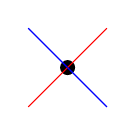
\begin{tikzpicture}[scale=0.5]
  \filldraw (0,0) circle (5pt);
  \draw[red] (0,0) -- (-1,-1);
  \draw[blue] (0,0) -- (-1,1);
  \draw[red] (0,0) -- (1,1);
  \draw[blue] (0,0) -- (1,-1);
  \end{tikzpicture}
  \captionsetup{justification=centering}
  \caption{Cross-over signature $\mathcal{C}$}
  \label{cross-over signature}
  \end{subfigure}
  \begin{subfigure}[t]{0.25\textwidth}
  \centering
  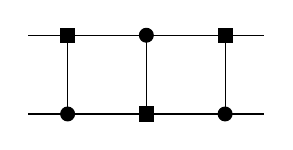
\begin{tikzpicture}[scale=0.5]
  \draw[black, very thick, fill=black] (-2.15,0.85) rectangle (-1.85,1.15);
  \filldraw (-2,-1) circle (5pt);
  \draw[black, very thick, fill=black] (-0.15,-1.15) rectangle (0.15,-0.85);
  \filldraw (0,1) circle (5pt);
  \draw[black, very thick, fill=black] (1.85,0.85) rectangle (2.15,1.15);
  \filldraw (2,-1) circle (5pt);
  \draw (-3,1) -- (3,1);
  \draw (-2,1) -- (-2,-1);
  \draw (0,1) -- (0,-1);
  \draw (2,1) -- (2,-1);
  \draw (-3,-1) -- (3,-1);
  \end{tikzpicture}
  \captionsetup{justification=centering}
  \caption{Cross-over gadget $G_4$}
  \label{G4}
  \end{subfigure}
  \begin{subfigure}[t]{0.18\textwidth}
  \centering
  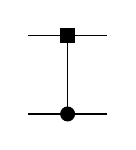
\begin{tikzpicture}[scale=0.5]
  \draw[black, very thick, fill=black] (-0.15,0.85) rectangle (0.15,1.15);
  \filldraw (0,-1) circle (5pt);
  \draw (0,-1) -- (0,1);
  \draw (1,1) -- (-1,1);
  \draw (-1,-1) -- (1,-1);
  \end{tikzpicture}
  \captionsetup{justification=centering}
  \caption{Component $A$}
  \label{G4A}
  \end{subfigure}
  \begin{subfigure}[t]{0.18\textwidth}
  \centering
  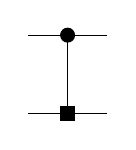
\begin{tikzpicture}[scale=0.5]
  \draw[black, very thick, fill=black] (-0.15,-1.15) rectangle (0.15,-0.85);
  \filldraw (0,1) circle (5pt);
  \draw (0,-1) -- (0,1);
  \draw (1,1) -- (-1,1);
  \draw (-1,-1) -- (1,-1);
  \end{tikzpicture}
  \captionsetup{justification=centering}
  \caption{$B = $ Up-Down flipped copy of $A$}
  \label{G4B}
  \end{subfigure}
  \captionsetup{justification=centering}
  \caption{Interpolate the cross-over signature $\mathcal{C}$}
\end{figure}

To prove Lemma~\ref{lemma:[1,a,1,a]}, let us define the cross-over  signature $\mathcal{C}$ of arity 4,  illustrated in Figure~\ref{cross-over signature}. It is 0-1 valued, and it takes value 1
iff the two  red dangling edges are equal and 
%(after being merged) represent an equality, as do 
the two blue dangling edges are equal; furthermore, it is a straddled signature where the two top dangling edges are to be connected to RHS externally and the two bottom dangling edges are to be connected to LHS externally. 
%%%%%%%%JYC omit the next segment in the para for the short version
In Figure~\ref{cross-over signature} only one vertex is present
pictorially.
However, when this signature is actually
implemented  or interpolated by some construction, the internal vertices that the two top  dangling edges are incident to
are LHS vertices; and
the  internal vertices that the  two bottom dangling edges 
are incident to
are RHS vertices.
%the same is true for the two bottom   dangling edges.
%We may consider the two top (resp.\ bottom) dangling edges are connected internally to LHS
%(resp.\ RHS) vertices.  (In Figure~\ref{cross-over signature} only one vertex is present; however when $\mathcal{C}$
%is implemented or interpolated, the vertices that the two top  dangling edges are incident to
%are distinct vertices; the same is true for the two bottom   dangling edges.)
%%% I need to say this, because later when i talk about having an edge intersecting many edges 
%% and use many copies of C, this is easier to say.

For later convenience, we will write the  signature matrix for $\mathcal{C}$
with
rows  (resp.\ columns)   indexed by $(b_1, b_2) \in \{0, 1\}^2$
corresponding to the dangling edges on the leftside (resp. rightside)
as it appears in Figure~\ref{cross-over signature} (not the LHS, RHS
designation according to the bipartiteness), 
with $b_1$ for the top  edge.
The signature matrix is $\mathcal{C} = \left( \begin{smallmatrix}
    1 & 0 & 0 & 0 \\
    0 & 0 & 1 & 0 \\
    0 & 1 & 0 & 0 \\
    0 & 0 & 0 & 1 
\end{smallmatrix}\right)$. Note that the signature matrix of $\mathcal{C}$ is invariant under a cyclic rotation by 90$^\circ$ of the graph in Figure~\ref{cross-over signature}. The importance of this cross-over signature is conveyed in the following lemma.
%which has been used implicitly among previous works.

We say a signature $f$ can be  planarly constructed or interpolated
if there is a polynomial time construction of planar gadgets or a sequence
of planar gadgets with external dangling edges conforming
to that of $f$ with respect to its bipartite specification,   such that 
the construction implements or interpolates $f$.
\begin{lemma}\label{lemma:cross-over}
For any signature sets $\mathcal{F}, \mathcal{G}$, if the cross-over signature $\mathcal{C}$ can be planarly constructed or interpolated, then $\holant{\mathcal{F}}{\mathcal{G}} \leq_{T} \plholant{\mathcal{F}}{\mathcal{G}}$.
\end{lemma}

\begin{proof}
Given any input signature grid of the problem $\holant{\mathcal{F}}{\mathcal{G}}$, we place it on the plane with possible edges intersecting each other at non-vertices. 
We may assume at most two edges intersect at any point, and the number of such intersections is  polynomially bounded.  
We replace each such intersection  by a copy of $\mathcal{C}$ as follows. 
Note that every
 edge connects a LHS
vertex with a RHS vertex.
Suppose an edge $e = \{u, v\}$ intersects consecutively $k \ge 1$  edges at non-vertices $x_1, \ldots, x_k$, 
where $u$ and $v$ are
from LHS and RHS, respectively. As we traverse from $u$ to $v$, for each $1 \le i \le k$ we label  R and L respectively
just as we enter and leave $x_i$. Labeling in this way for every edge having
such intersections, we find that locally at each intersection point,
cyclically two consecutive edges are labeled R and the other two consecutive edges are labeled L.
This is because at each local intersection point each pair of
incident edges that are \emph{not} cyclically consecutive are always labeled with distinct R $\ne$ L.
A moment reflection shows that the signature
$\mathcal{C}$ can always be used 
with a suitable 
 rotation at each intersection, while
respecting the bipartite structure.
%cyclically two consecutive input wires are connected to LHS and the other
%two consecutive input wires are connected to RHS, which is exactly the case for each crossing in the original signature grid due to the bipartite structure.
We thus obtain an input of the problem $\plholant{\mathcal{F}}{\mathcal{G}}$ with Holant value unchanged.
\end{proof}

% \begin{proof}
% Given any input signature grid of the problem $\holant{\mathcal{F}}{\mathcal{G}}$, we place it on the plane with possible edges intersecting each other at non-vertices. 
% We may assume at most two edges intersect at any point, and the number of such intersections is  polynomially bounded.  
% We replace each such intersection  by a copy of $\mathcal{C}$ as follows. 
% Note that every
%  edge connects a LHS
% vertex with a RHS vertex.
% Suppose an edge $e = \{u, v\}$ intersects consecutively $k \ge 1$  edges at non-vertices $x_1, \ldots, x_k$, 
% where $u$ and $v$ are
% from LHS and RHS, respectively. As we traverse from $u$ to $v$, for each $1 \le i \le k$ we label  R and L respectively
% just as we enter and leave $x_i$. Labeling in this way for every edge having
% such intersections, we find that locally at each intersection point,
% cyclically two consecutive edges are labeled R and the other two consecutive edges are labeled L.
% This is because at each local intersection point each pair of
% incident edges that are \emph{not} cyclically consecutive are always labeled with distinct R $\ne$ L.
% A moment reflection shows that the signature
% $\mathcal{C}$ can always be used 
% with a suitable 
%  rotation at each intersection, while
% respecting the bipartite structure.
% We thus obtain an input of the problem $\plholant{\mathcal{F}}{\mathcal{G}}$ with Holant value unchanged.
% \end{proof}

%We are now ready to prove Lemma~\ref{lemma:[1,a,1,a]}.

We are now ready to prove Lemma~\ref{lemma:[1,a,1,a]}.

\begin{proof}[Proof of Lemma~\ref{lemma:[1,a,1,a]}]
When $a=0$ or $\pm1$, the problem is in the affine class or degenerate, respectively, and thus in $\operatorname{FP}$ (see~\cite{cai2017complexity} for details of the algorithms). Assume $a \neq 0 $ and $a \neq \pm 1$.
The problem $\holant{[1,a,1,a]}{(=_3)}$ without the planar restriction
is shown to be \numP-hard in \cite{CaiFL21}. By Lemma~\ref{lemma:cross-over}, it suffices to show we can interpolate the cross-over signature $\mathcal{C}$. 

Consider
the gadget $G_4$ in Figure~\ref{G4} where we place 
the signature $[1,a,1,a]$ at the square vertices
and $=_3$ at the circle vertices. Note that $G_4$ is a straddled signature
with the two dangling edges at the top (reps. bottom) to be connected externally
to the RHS (reps.  LHS), just like the cross-over signature $\mathcal{C}$. After normalization 
by a constant $a+a^2 \ne 0$, the signature matrix of $G_4$  is  $\left(\begin{smallmatrix}
    z & 1 & 1 & 1 \\
    1 & 1 & z & 1 \\
    1 & z & 1 & 1 \\
    1 & 1 & 1 & z
\end{smallmatrix}\right)$,
where $z = \frac{1+a^3}{a+a^2} = a + a^{-1} - 1$.
As $a \ne \pm 1$, 
if $a >0$  then
$z =(a^{1/2} - a^{-1/2})^2 +1 > 1$, and if 
$a<0$  then $z = - (|a| + |a|^{-1}) - 1= -(|a|^{1/2} - |a|^{-1/2})^2 -3 
<-3$.
Here the rows  (resp. columns)  are  indexed by $(b_1, b_2) \in \{0, 1\}^2$ in lexicographic order
corresponding to the dangling edges on the leftside (resp. rightside,
as it appears in Figure~\ref{G4}), 
with $b_1$ for the top  edge.
This can be  verified by first computing the signatures for $A$ and $B$ in
Figures~\ref{G4A} and~\ref{G4B},
$A = \left( \begin{smallmatrix}
    1 & 0 & a & 0 \\
    0 & a & 0 & 1 \\
    a & 0 & 1 & 0 \\
    0 & 1 & 0 & a
\end{smallmatrix}
\right)$,
and  $B =\left(\begin{smallmatrix}
    1 & a & 0 & 0 \\
    a & 1 & 0 & 0 \\
    0 & 0 & a & 1 \\
    0 & 0 & 1 & a
\end{smallmatrix}
\right)$ is obtained from $A$ by exchanging both  middle two rows and 
 middle two columns. Then we have $G_4 = A \cdot B \cdot A$, as a matrix product.
Notice that the ``shape" of $G_4$ looks just like $\mathcal{C}$ if we replace 1 by 0, and $z$ by 1. We will exploit this remarkable coincidence
in our proof below.
Note also that the signature matrix of $G_4$ is invariant under cyclic rotations of the gadget.

Now we define a sequence of gadgets $\Gamma_{2s+1}$ of linear size,
which is a sequential composition of
$2s+1$ sub-gadgets, where for odd index $i=1, 3, \ldots, 2s+1$
we use  $G_4$, and for even index $i=2, 4, \ldots, 2s$
we use a  $180^\circ$-rotated copy of  $G_4$, and 
we merge the rightside two edges
of the $i$th sub-gadget with the leftside two edges
of the $(i+1)$th sub-gadget.
This  sequential composition  satisfies
the bipartite restriction. As the
rotated copy of  $G_4$ has the 
same signature matrix as that of $G_4$,
the signature matrix of $\Gamma_{2s+1}$  is $G_4^{2s+1}$,
the $(2s+1)$th power of $G_4$.
We can show
that it has the form (after normalization) 
$\Gamma_{2s+1} = \left(\begin{smallmatrix}
    x_s & 1 & 1& 1 \\
    1 & 1 & x_s & 1 \\
    1 & x_s & 1 & 1\\
    1 & 1 & 1 & x_s
\end{smallmatrix}\right)$,
where $\{x_s\}_{s \ge 0}$ are defined by a recurrence, with $x_0 = z$ and \[x_{s+1} = \frac{6+6z+3x_s+z^2\cdot x_s}{7+4z+z^2+2x_s+2z\cdot x_s}. \]
%The partial derivative of $x_{s+1}$ with respect to $x_s$
%is $\frac{\partial x_{s+1}}{\partial x_{s}} = \frac{(z-1)^2(z+3)^2}{(7+4z+z^2+2x_s+4z\cdot x_s)^2} >0$. Therefore $x_{s+1}$ is strictly increasing with respect to $x_{s}$.
%It follows that $x_s$'s are pairwise distinct.

We are going to show that $x_s$'s are pairwise distinct. 
First suppose $a >0$. We have $x_{s+1} - 1
=\frac{(z-1)^2(x_s -1)}{7+4z+z^2+2x_s+2z\cdot x_s}$,
which
shows inductively that $x_s > 1$
 for all $s \in \mathbb{N}$, as the denominator is clearly positive. 
 Next, $\frac{x_{s+1} - 1}{x_s -1} = \frac{(z-1)^2}{(z+2)^2 + 3+2x_s(z+1)} <1$, as $x_s, z>1$.
 %Next, $x_{s+1}-x_s<0$ iff $6+6z < x_s\cdot (4+4z+2x_s+2z x_s)$, which is true since $x_s > 1$ for all $s \in \mathbb{N}$.
 %It follows that the sequence $x_s$'s is strictly decreasing
 It follows that $x_{s+1}  < x_s$
 and hence pairwise distinct.
 Now suppose $a <0$. Inductively assume $x_s < -3$, which is true
 at $x_0 = z < -3$.
 We have $x_{s+1} + 3
 =\frac{(z+3)^2 (x_s +3)}{7+4z+z^2+2x_s+2z\cdot x_s}$.
 The denominator $7+4z+z^2+2x_s+2z\cdot x_s
 =(z+2)^2 +3 + 2 (z+1) x_s >0$, as $z <-3$ and inductively also $x_s <-3$.
 Then we  have $x_{s+1} + 3 <0$ since $x_s +3 < 0$.
 Now the denominator is $(z+2)^2 +3 + 2 (z+1) x_s > |z+2|^2 > |z+3|^2$
 as $z <-3$. Hence $\frac{x_{s+1} + 3}{x_s +3} =
 \frac{(z+3)^2}{(z+2)^2 +3 + 2 (z+1) x_s} <1$.
And so,  $x_{s+1} > x_s$, and  in particular they are pairwise distinct.
 %in fact x_{s+1} > x_s


 

%First suppose $a >0$. We first prove $x_s > 1$ for any $s \in \mathbb{N}$ by induction. When $s=0$, we have $x_0=z>1$. Suppose this is true up to $s = k$ for some $k\in \mathbb{N}$. Then $x_{k+1} > 1$ iff $6+6z+3x_k+z^2 x_k > 7 + 4z+z^2+2x_k+2z x_k$ iff $(z-1)^2\cdot (x_k-1) > 0$, which is true by the inductive hypothesis. We now show $x_s$'s are pairwise distinct by showing the sequence $x_s$'s is strictly decreasing. Indeed, the difference $x_{s+1}-x_s<0$ iff $6+6z < x_s\cdot (4+4z+2x_s+2z x_s)$, which is true since $x_s > 1$ for any $s \in \mathbb{N}$.

Note also that the number of bits required to represent $x_s$'s is polynomially bounded in the size of the input
because $x_s$'s come from, by definition, sums of at most $2^{n^{O(1)}}$ terms, each a product of $n^{O(1)}$ factors. 
%%% JYC i changed to "come from" because there was a normailization step

Given any signature grid $\Omega$ where the cross-over signature $\mathcal{C}$ appears $n$ times, we construct signature grids $\Omega_s$, $0 \leq s \leq n$,
by replacing each copy of $\mathcal{C}$ by $\Gamma_{2s+1}$ while respecting
the bipartite restrictions. 
 We now stratify the assignments in the Holant sum for $\Omega$ according to the number $i$, $0 \leq i \leq n$, of total times that the input of $\mathcal{C}$ is (0,0,0,0), (1,0,1,0), (0,1,0,1), or (1,1,1,1) in cyclic order (these are the only inputs
 to  $\mathcal{C}$ with nonzero evaluations). Let $c_i$ be the sum over all corresponding assignments of the products from other signatures with this restriction of $i$. Then we have 
$\operatorname{Holant}(\Omega) = c_n$,
and
\begin{equation}\label{Vandermonde}
   \operatorname{Holant}(\Omega_s) = \sum\limits_{i=0}^n x^i_s \cdot c_i.
\end{equation}
Since  $x_s$'s are pairwise distinct, (\ref{Vandermonde}) is a full ranked
Vandermonde system, and we can solve for all $c_i$ in polynomial time, and 
in particular compute $c_n$, from the values of $\operatorname{Holant}(\Omega_s)$, $0 \leq i \leq n$.
\end{proof}



%We are now ready to prove the following basic lemma.

%\begin{figure}[ht]
%  \centering
%  \begin{subfigure}[b]{0.3\textwidth}
%  \centering
%  \begin{tikzpicture}[scale=0.5]
%  \filldraw (2,0) circle (5pt);
%  \draw[black, very thick, fill=black] (-0.15,-0.15) rectangle (0.15,0.15);
%  \draw (0,0) .. controls (0.5,0.75) and (1.5,0.75) .. (2,0); 
%  \draw (0,0) .. controls (0.5,-0.75) and (1.5,-0.75) .. (2,0); 
%  \draw (0,0) -- (-1.5,0);
%  \draw (2,0) -- (3.5,0);
%  \end{tikzpicture}
%  \captionsetup{justification=centering}
%  \caption{Binary  straddled  gadget $G_1$}
%  \label{some gadgets G_1}
%  \end{subfigure}
%  \begin{subfigure}[b]{0.3\textwidth}
%  \centering
%  \begin{tikzpicture}[scale=0.5]
%  \draw[black, very thick, fill=black] (-0.15,-0.15) rectangle (0.15,0.15);
%  \filldraw (-1,-0.5) circle (5pt);
%  \filldraw (1,-0.5) circle (5pt);
%  \filldraw (0,1) circle (5pt);
%  \draw[black, very thick, fill=black] (-0.15,-2.15) rectangle (0.15,-1.85);
%%  \filldraw (0,-2) circle (5pt);
%  \draw[black, very thick, fill=black] (-2.15,0.85) rectangle (-1.85,1.15);
%%  \filldraw (-2,1) circle (5pt);
%  \draw[black, very thick, fill=black] (1.85,0.85) rectangle (2.15,1.15);
%%  \filldraw (2,1) circle (5pt);
%  \draw (0,0) -- (-1,-0.5);
%  \draw (0,0) -- (1,-0.5);
%  \draw (0,0) -- (0,1);
%  \draw (0,-2) -- (-2,1);
%  \draw (0,-2) -- (2,1);
%  \draw (-3,1) -- (3,1);
%  \draw (0,-2) -- (0,-3);
%  \end{tikzpicture}
%  \captionsetup{justification=centering}
%  \caption{Ternary gadget $G_2$}
%  \end{subfigure}
%  \begin{subfigure}[b]{0.3\textwidth}
%  \centering
%  \begin{tikzpicture}[scale=0.5]
%  \filldraw (-1.5,0) circle (5pt);
%  \filldraw (1.5,0) circle (5pt);
%% \filldraw (0,0) circle (5pt);
%  \draw[black, very thick, fill=black] (-0.15,-0.15) rectangle (0.15,0.15);
%% \filldraw (-3,0) circle (5pt);
%  \coordinate (x1) at (-3,0.3);
%  \coordinate (y1) at (-3.25,-0.15);
%  \coordinate (z1) at (-2.75,-0.15);
%  \filldraw[draw=black, fill=black] (x1) -- (y1) -- (z1) -- cycle;
%% \filldraw (1.5,1.5) circle (5pt);
%  \coordinate (x2) at (1.25,1.35);
%  \coordinate (y2) at (1.75,1.35);
%  \coordinate (z2) at (1.5,1.8);
%  \filldraw[draw=black, fill=black] (x2) -- (y2) -- (z2) -- cycle;
%  \draw (-3,0) -- (-1.5,0);
%  \draw (1.5,0) -- (1.5,1.5);
%  \draw (1.5,0) -- (0,0);
%  \draw (0,0) .. controls (-0.5,0.75) and (-1,0.75) .. (-1.5,0); 
%  \draw (0,0) .. controls (-0.5,-0.75) and (-1,-0.75) .. (-1.5,0); 
%  \draw[very thick, dotted] (-3,0) -- (-4,0);
%  \draw[very thick, dotted] (1.5,1.5) -- (1.5,2.5);
%  \draw (1.5,0) -- (2.5,0);
%  \end{tikzpicture}
%  \captionsetup{justification=centering}
%  \caption{Ternary gadget $G_3$}
%  \end{subfigure}
%  \caption{Some gadgets, where squares are $[1,a,b,c]$ on LHS and circles are $(=_3)$ on RHS}
%  \label{some gadgets}
%\end{figure}




Hereafter, we say $[1,a,b,c]$ is \numP-hard or in FP to mean the problem $\plholant{[1,a,b,c]}{(=_3)}$ is \numP-hard or in FP. We shall invoke the following theorem in~\cite{MKJYC} when proving our results:
\begin{theorem}[Kowalczyk \& Cai] \label{previous 2-3}
Suppose $a,b \in \mathbb{C}$, and let $X = ab$, $Z = \left( \frac{a^3+b^3}{2} \right)^2$. Then $\plholant{[a,1,b]}{\left(=_3\right)}$ is \numP-hard except in the following cases, for which the problem is in $\operatorname{FP}$.

\begin{enumerate}
\item $X=1$;
\item $X=Z=0$;
\item $X=-1$ and $Z=0$;
\item $X=-1$ and $Z=-1$;
\item $X^3 = Z$.
\end{enumerate}
\end{theorem} 

By restricting Theorem~\ref{previous 2-3} to real numbers, we have the following corollary.

\begin{corollary} \label{2-3}
Suppose $a,b \in \mathbb{R}$, then $\plholant{[a,1,b]}{\left(=_3\right)}$ is \numP-hard except in the following cases, for which the problem is in $\operatorname{FP}$.

\begin{enumerate}
\item $ab=1$;
\item $a=1$ and $b=-1$;
\item $a=-1$ and $b=1$;
\item $a=b$.
\end{enumerate}
\end{corollary} 


\begin{figure}[ht] 
\centering
  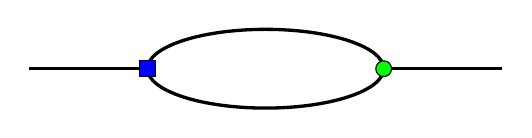
\begin{tikzpicture}% G1
        % \draw[step=1cm, green,very thin](-1.9,-1.9) grid (5.9,5.9);
        % \draw[thick, ->] (0,0) -- (4.5,0) node[anchor=north west] {x axis};
        % \draw[thick, ->] (0,0) -- (0,4.5) node[anchor=south east] {y axis};
        \draw [very thick] (-1,0.5) -- (0.5,0.5);
        
        % \draw[very thick] (3.5, 1) arc (45:135:2.2cm);
        % \draw[very thick] (0.5, 0) arc (225:315:2.2cm);
        \draw[very thick] (2,0.5) ellipse (1.5cm and 0.5cm);
        \draw[very thick] (3.5,0.5) -- (5,0.5);
        \filldraw[fill= blue] (0.4,0.4) rectangle (0.6,0.6);
        \filldraw[fill=green] (3.5,0.5) circle (0.1cm);
    \end{tikzpicture}
    \captionsetup{justification=centering}
    \caption{Gadget $G_1$}
  \label{f1}
\end{figure}


Consider the binary straddled gadget $G_1$ in Figure \ref{f1}. 
Parallel edges are allowed. Its signature is $G_1=\left[\begin{smallmatrix} 1 & b \\ a & c \end{smallmatrix}\right]$, where  $G_1(i,j)$ (at row $i$ column $j$) is the value of this gadget when the left dangling edge (from the ``square") and the right dangling edge (from the ``circle" $(=_3)$) are assigned $i$ and $j$ respectively, for $i,j \in\{0,1\}$.
%The following lemma  can be proved similarly
%  as Lemma 3.1 in~\cite{fan2020dichotomy}.
Iterating $G_1$ sequentially $k$ times is represented by the
matrix power $G_1^k$. It turns out that it is very useful
 either to produce directly  or to obtain by interpolation
a rank \emph{deficient} straddled signature, which would in most cases allow us to obtain unary signatures on either side.
With unary signatures we can connect to a ternary signature
to produce binary signatures on one side and then apply
Corollary~\ref{2-3}. 

The following lemma is proved in~\cite{CaiFL21}.

\begin{lemma} \label{3.1.1}
Given the binary straddled signature $G_1=\left[\begin{smallmatrix} 1 & b \\ a & c \end{smallmatrix}\right]$, we can interpolate the degenerate binary straddled signature $\left[\begin{smallmatrix}y & xy \\ 1 & x\end{smallmatrix}\right]$,
provided that $c\neq ab$, $a\neq 0$, $\Delta =\sqrt{(1-c)^2 + 4ab} \neq 0$ and $\frac{\lambda}{\mu}$ is not a root of unity, where
$\lambda=\frac{-\Delta+(1+c)}{2}$, $\mu=\frac{\Delta+(1+c)}{2}$ are the
 two eigenvalues,  
 and $x=\frac{\Delta-(1-c)}{2 a}$ and $y=\frac{\Delta+(1-c)}{2 a}$.
\end{lemma}


Given a degenerate binary straddled signature, we want to use it as unary signatures \emph{in a planar way}. It is only in this step that we need our P3EM theorem. More concretely, in the next lemma we show how we can \emph{essentially} separate a binary straddled signature to get a unary
signature.


\begin{lemma} \label{3.1.2}
For $\PlHolant( \, [1,a,b,c] \, | =_3)$,\ 
%problem $[1,a,b,c]$,\ 
$a,b,c \in \mathbb{Q}$, $a\neq 0$,  with the availability of the binary degenerate straddled signature $\left[\begin{smallmatrix}y & xy \\ 1 & x\end{smallmatrix}\right]$ where 
$x=\frac{\Delta-(1-c)}{2 a}$,  $y=\frac{\Delta+(1-c)}{2 a}$ and $\Delta=\sqrt{(1-c)^2 + 4ab}$, we have the following reductions
%problem $[1,a,b,c]$,\ 
\begin{enumerate}
    \item $\PlHolant ( \, [1+ax,a+bx,b+cx] \, | =_3) \leq_T \PlHolant ( \, [1,a,b,c] \, | =_3)$ except for 2 cases:
    %(by Remark under Lemma \ref{3.1.2}, the two cases happen when $y=-1$)
    %: 
    $[1,a,a,1]$, $[1,a,-1-2a, 2+3a]$;
    \item $ \PlHolant ( \, [1,a,b,c] \, | [y,0,1]) \leq_T \PlHolant ( \, [1,a,b,c] \, | =_3)$.
    
\end{enumerate}  
\end{lemma}

\begin{figure}[ht]
    \centering
    \begin{subfigure}[b]{0.3\textwidth}
    \centering
    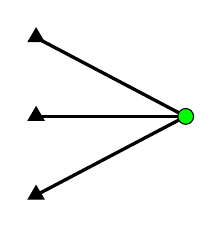
\begin{tikzpicture}  % h1
        \draw[very thick] (0.3,5.05) -- (2.2,4.05);
        \draw[very thick] (0.3,4.05) -- (2.2,4.05);
        \draw[very thick] (0.3,3.05) -- (2.2,4.05);
        \filldraw[fill=black] (0.3,5.17)--(0.2,5)--(0.4,5)--cycle;
        \filldraw[fill=black] (0.3,4.17)--(0.2,4)--(0.4,4)--cycle;
        \filldraw[fill=black] (0.3,3.17)--(0.2,3)--(0.4,3)--cycle;
        \filldraw[fill=green] (2.2, 4.05)circle(0.1);
    \end{tikzpicture}
    \captionsetup{justification=centering}
    \caption{$g_1$}
    \label{h1}
    \end{subfigure}
    \begin{subfigure}[b]{0.3\textwidth}
    \centering
    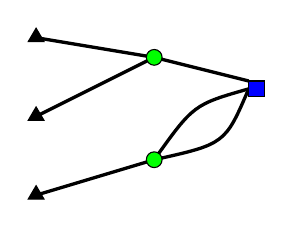
\begin{tikzpicture}  %h2
        \draw[very thick] (0.3,5.05)--(1.8,4.8);
        \draw[very thick] (0.3,4.05)--(1.8,4.8);
        \draw[very thick] (0.3,3.05)--(1.8,3.5);
        \draw[very thick] (1.8,4.8) -- (3,4.5);
        \draw[very thick] (1.8,3.5).. controls (2.3, 4.2) ..(3,4.4);
        \draw[very thick] (1.8,3.5) .. controls (2.7, 3.7)..(3,4.4);
        \filldraw[fill=black] (0.3,5.17)--(0.2,5)--(0.4,5)--cycle;
        \filldraw[fill=black] (0.3,4.17)--(0.2,4)--(0.4,4)--cycle;
        \filldraw[fill=black] (0.3,3.17)--(0.2,3)--(0.4,3)--cycle;
        \filldraw[fill=green] (1.8,4.8) circle (0.1);
        \filldraw[fill=green] (1.8,3.5) circle (0.1);
        \filldraw[fill=blue] (3,4.3)rectangle(3.2,4.5);
    \end{tikzpicture}
    \captionsetup{justification=centering}
    \caption{$g_2$}
    \label{h2}
    \end{subfigure}
    \captionsetup{justification=centering}
    \caption{Two gadgets where each triangle represents the unary gadget $[y,1]$}
    \label{3g4y1}
\end{figure}


\begin{figure}[ht]
    \centering
    \begin{subfigure} [b] {0.3\textwidth}
    \centering
    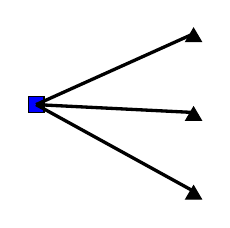
\begin{tikzpicture}  % e1
        \filldraw[fill=blue] (0.2,2.2) rectangle (0.4,2.4);
        \filldraw[fill=black] (2.3,3.27)--(2.2,3.1)--(2.4,3.1)--cycle ;
        \filldraw[fill=black] (2.3,2.27)--(2.2,2.1)--(2.4,2.1)--cycle;
        \filldraw[fill=black] (2.3,1.27)--(2.2,1.1)--(2.4,1.1)--cycle;
        \draw[very thick] (0.3,2.3)--(2.3,3.2);
        \draw[very thick] (0.3,2.3)--(2.3,2.2);
        \draw[very thick] (0.3,2.3)--(2.3,1.2);
    \end{tikzpicture}
    \captionsetup{justification=centering}
    \caption{$f_1$}
    \label{e1}
    \end{subfigure}
        \hspace{10pt}
    \begin{subfigure}  [b]{0.3\textwidth}
    % \centering
    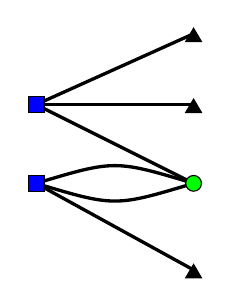
\begin{tikzpicture}   %e2
        \filldraw[fill=black] (2.3,5.27)--(2.2,5.1)--(2.4,5.1)--cycle;
        \filldraw[fill=black] (2.3,4.37)--(2.2,4.2)--(2.4,4.2)--cycle;
        \filldraw[fill=black] (2.3,2.27)--(2.2,2.1)--(2.4,2.1)--cycle;
        
        
        \draw[very thick] (0.3,4.3) -- (2.3,5.2);
        \draw[very thick] (0.3,4.3)--(2.3,4.3);
        \draw[very thick] (0.3,4.3)--(2.3,3.3);
        \draw[very thick] (0.3,3.3) ..controls (1.3,3.6)..  (2.3, 3.3);
        \draw[very thick] (0.3,3.3) .. controls (1.3, 3.0).. (2.3, 3.3);
        \draw[very thick] (0.3,3.3) -- (2.3, 2.2);
        \filldraw[fill=blue] (0.2,4.2) rectangle (0.4,4.4) ;  % 0.3, 4.3
        \filldraw[fill=blue] (0.2,3.2) rectangle (0.4,3.4) ;  % 0.3, 3.3
        \filldraw[fill=green] (2.3,3.3) circle (0.1cm) ;
    \end{tikzpicture}
    \captionsetup{justification=centering}
    \caption{$f_2$}
    \label{e2}
    \end{subfigure}
    \hspace{10pt}
    \begin{subfigure}  [b]{0.3\textwidth}
    \centering
    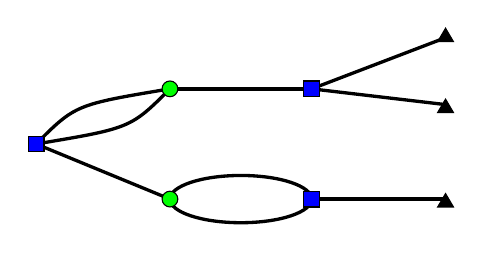
\begin{tikzpicture}  %e4
        \draw[very thick] (0.3,4.3)..controls(0.8,4.8)..(2,5);
        \draw[very thick] (0.3,4.3)..controls(1.5, 4.5 )..(2,5);
        \draw[very thick] (0.3,4.3)--(2,3.6);
        \draw[very thick] (3.8,5)--(2,5);
        
        \draw[very thick] (3.8,5)--(5.5,5.65);
        \draw[very thick] (3.8,5)--(5.5,4.8);
        \draw[very thick] (3.8,3.6)--(5.5,3.6);
        
        \draw[very thick]  (2.9, 3.6) ellipse(0.9 and 0.3); %(2,3.6) -- (3.8,3.6)
        \filldraw[fill=blue] (0.2,4.2) rectangle(0.4,4.4); %(0.3,4.3)
        \filldraw[fill=green] (2,5) circle (0.1cm);     % (2,5)
        \filldraw[fill=green] (2,3.6) circle(0.1cm);    % (2,3.6)
        \filldraw[fill=blue] (3.7,4.9) rectangle (3.9,5.1);   %(3.8,5)
        \filldraw[fill=blue] (3.7,3.5) rectangle (3.9, 3.7);  % (3.8, 3.6)
        \filldraw[fill=black] (5.5,5.77)--(5.4,5.6)--(5.6,5.6)--cycle; 
        \filldraw[fill=black] (5.5,4.87)--(5.4,4.7)--(5.6,4.7)--cycle; 
        \filldraw[fill=black] (5.5,3.67)--(5.4,3.5)--(5.6,3.5)--cycle; 
    \end{tikzpicture}
    \captionsetup{justification=centering}
    \caption{$f_3$}
    \label{e3}
    \end{subfigure}
    \captionsetup{justification=centering}
    \caption{Three gadgets where each triangle represents the unary gadget $[1,x]$}
    \label{4g41x}
\end{figure}

\begin{proof}
The signature $[1+ax,a+bx,b+cx]$ is the binary signature obtained by connecting $[1,a,b,c]$ on LHS with $[1,x]$ on RHS. For simplicity, we denote $f : = [1,a,b,c]$ and $f^{\flat} := [1+ax,a+bx,b+cx]$.


To prove the first reduction $\PlHolant ( \,  f^{\flat}\, | =_3) \leq_T \PlHolant ( \, f \, | =_3)$, 
consider any input instance of the LHS  problem.  Let 
$G$ be its underlying 2-3 bipartite plane graph. 
We may assume
$G$ is connected, as the Holant value of $G$ is 
the product of the Holant values of its connected components.
We can view $G$ as the edge-vertex incidence graph of
a plane 3-regular graph 
$G'$, where every vertex of degree 2 in $G$ on the LHS is viewed
as an edge in $G'$. One can also
obtain $G'$ 
by merging the two edges
incident to every vertex of degree 2 in $G$.
If $G'$ is isomorphic to one of the two exceptions in Theorem~\ref{thm:P3EM}, then the size of $G$ is constant and we can compute the Holant value directly. Otherwise, we construct an input of the RHS problem as follows. 
We first obtain the degenerate binary straddled signature $D = \left[\begin{smallmatrix}y & xy \\ 1 & x\end{smallmatrix}\right]$
in $\plholant{[1,a,b,c]}{(=_3)}$. 
Then for every edge of $G'$, which is
assigned  the binary
signature $f^{\flat}$,
%$[1+az,a+bz,b+cz]$,
we replace it by a copy of $[1,a,b,c]$ and  connecting it
with
the edge of $D$ that corresponds to $[1,x]$.
This leaves 
1 dangling edge from each copy of $D$, each 
edge functionally equivalent to
a unary $[y,1]$ on LHS. They need to be connected to other $(=_3)$ signatures in a planar way.
Now we apply Theorem~\ref{thm:P3EM} to the
3-regular plane graph $G'$, which constructively
assigns every edge of $G'$ one of the two incident
faces such that we have a P3EM. We then add a suitable number
of $(=_3)$ and $f$ in each face
and connect them to \emph{exactly} 3 copies of
$[y,1]$ as shown in Figures \ref{h1} and  \ref{h2}.
Theorem~\ref{thm:P3EM} guarantees that
this can be done in a planar way.
Each connection produces a multiplicative factor
$g_1 =y^3 + 1$ in Figure \ref{h1} and a multiplicative factor $g_2 = y^3 + by^2+ay+c$ in Figure \ref{h2}. It can be directly checked that\footnotemark \footnotetext{We use Mathematica to solve the system of equation \begin{equation*}\begin{cases}
g_1 = y^3 + 1 = 0\\
g_2 = y^3 + by^2+ay+c = 0\\
y=\frac{\Delta+(1-c)}{2 a}
    \end{cases}
\end{equation*}
%and for each equation to be zero we set both real and imaginary parts to be zero. 
The empty solution of the system is proved by cylindrical decomposition, an algorithm for Tarski's theorem on real-closed fields.}, for $y=\frac{\Delta+(1-c)}{2 a}$, at least one of these factors is nonzero unless $y=-1$, and in that case the signature has the form $[1,a,a,1]$ or $[1,a,-2a-1,3a+2]$.
The proof of the  reduction is complete.% Some more work is
%needed to prove the Lemma; see the appendix for details.


For the reduction $ \PlHolant ( \, [1,a,b,c] \, | [y,0,1]) \leq_T \PlHolant ( \, [1,a,b,c] \, | =_3)$, we use the same P3EM argument as above. Therefore it suffices to ``absorb'' those dangling unaries $[1,x]$ to produce some nonzero factor. We claim that at least one of the connection gadgets in Figures \ref{e1}, \ref{e2}, and \ref{e3} creates a nonzero global factor. 
% MK8
The factors of these four gadgets are \begin{equation*}\begin{cases}
f_1 = cx^3+3bx^2+3ax+1 \\
f_2=(ab+c)x^3+ (3bc+2a^2+b)x^2 +(2b^2+ac + 3a)x+ab+1\\
\begin{split}f_3 = 
    & (ab+2abc+c^3)x^3+(2a^2+b+2a^2c+3ab^2+bc+3b^2c)x^2 \\
    & +(3a+3a^2b+ac+2b^2+2b^2c+ac^2)x+1+2ab+abc
\end{split}
    \end{cases}
\end{equation*} respectively.
% and $f_5=(a^3+2abc+c^3)x^3 + (3a^2+2bc+2ab^2+2a^2c+3bc^2)x^2 + (3a+2ac+2a^2b+2b^2+3b^2c)x+(1+2ab+b^3))$,
 By setting the three formulae to be 0 simultaneously together with the condition $x=\frac{\Delta-(1-c)}{2 a}$, with $a\neq 0$, $a,b,c\in\mathbb{Q}$, we found that there is no common solution. The proof is now complete.
% : $[1,a,b,c]=[1,-1,-2,0]$ and $x$ is one of the root for equation $5x^9-x^6-x^3+1=0$. But actually, for $[1,-1,-2,0]$, we can interpolate binary straddled signature $\left(\begin{array}{ll}-2 & 2 \\ 1 & -1\end{array}\right)$ by Leamma \ref{3.1.1}. The $x$ here is $-1$ and so we can use it with $f_1$ to generate a global factor $-2$. On all other cases, 
\end{proof}

% i rewrote yur a' by x, b' by y
We note that signatures of the form $[3x+y,-x-y,-x+y,3x-y]$ for some $x,y$ are exactly either of the form $[1,a,-2a-1, 3a+2]$ 
after normalization, or of the form
%$[0,2a,-4a,6a]$ 
$[0,a,-2a,3a]$, for some $a$. 
%Conversely, any signature 
%of the form  $[1,a,-2a-1, 3a+2]$ is of the former type.
%%% no need to give this derivation below.
%Indeed, if $3a'+b' = 0$, then the signature is $[0,2a',-4a',6a']$. If $3a'+b'\neq 0$, then we normalize the signature by dividing $3a'+b'$ to get $[1,\frac{-a'-b'}{3a'+b'}, \frac{-a'+b'}{3a'+b'}, \frac{3a'-b'}{3a'+b'}]$ and set $a = \frac{-a'-b'}{3a'+b'}$. A direct calculation shows that the signature is now $[1,a,-2a-1,3a+2]$.


% We note that the form $[1,a,-2a-1, 3a+2]$ and the form $[3a'+b',-a'-b',-a'+b',3a'-b']$ are equivalent in expressive power. Indeed, one can easily check that $-2(-a'-b') - (3a'+b') = -a'+b'$ and $3(-a'-b') +2(3a'+b') = 3a'-b'$. Reversely, setting $a' = \frac{1+a}{2}$ and $b' = \frac{-(3a+1)}{2}$ yields $[3a'+b',-a'-b',-a'+b',3a'-b'] = [1,a,-2a-1, 3a+2]$.


\begin{remark}\label{remark8}
Just before Lemma~\ref{y11x} we stated that we could
\emph{essentially} separate a binary straddled signature to get a unary.
This statement is delicate. 
Getting unrestricted use of the unary $[1, x]$ on RHS would be
$\plholant{f}{(=_3), [1,x]}$.
The following two problems are equivalent.
$$\plholant{f, f^{\flat}}{(=_3)}
\equiv_T
\plholant{f}{(=_3), [1,x]}.
$$
This is because for the second problem, every occurrence of
$[1,x]$ is connected to $f$ to produce $f^{\flat}$,
and conversely for  the first problem, every occurrence of
$f^{\flat}$ can be replaced by connecting a copy of $f$  with
$[1,x]$.
However, we do not claim that the problem $\plholant{f}{(=_3), [1,x]}$ is reducible to
$\plholant{f}{(=_3)}$, which 
%would be 
is the following
stronger reduction than what we showed:
$$\plholant{f, f^{\flat}}{(=_3)} \leq_{T} \plholant{f}{(=_3)}.$$
%%%%JYC this sentence is not clear to me what it means.
% as is the in any instance of the LHS problem of course each [1,z] is connected to some copy of [1,a,b,c].
The issue is that now the 
 input graph for the LHS problem is not an edge-vertex incidence graph for a 3-regular plane graph, and so
we cannot apply Theorem~\ref{thm:P3EM} as before. 
If we merge the two incident
edges of all degree 2 vertices (assigned the binary
signature $f^{\flat}$) we do get a planar 3-regular graph.
But this graph may still have degree 3 vertices labeled $f$,
and not every edge comes from merging a degree 2 vertex that
was labeled $f^{\flat}$. Thus,
not every edge participates in a 3-way perfect matching.
In summary, a degenerate binary straddled signature is not completely equivalent to a unary $[1,x]$ on RHS.
We further remark  that, if this were true, we would have
a much simpler proof of Theorem~\ref{thm:[0,1,0,0]}.
\end{remark}

\begin{remark}
Reader should think of Lemma 9 mainly as an illustration of what we will call the \emph{P3EM argument}. The main take-away is that we can separate a degenerate binary straddled signature to get unaries so long as we use one of them on \emph{every} ternary signature on one side and the remaining dangling unaries can be absorbed to create a nonzero global factor. For example, in the proof of Theorem \ref{g1works1}, we are in fact using the gadget depicted in Figure~\ref{non_li}. For the sake of simplicity for presentation, we will say ``interpolate'' $[1,x]$ on RHS or $[y,1]$ on LHS hereafter while the reader is welcome to check the delicate issue in Remark~\ref{remark8} is taken care.
\end{remark}


The following proposition is proved in~\cite{CaiFL21}.

\begin{proposition} \label {g1-rou}
For $G_1 = \left[\begin{smallmatrix}1 & b \\ a & c\end{smallmatrix}\right]$, with $a,b,c \in \mathbb{Q}$, if it is non-singular (i.e., $c \ne ab$), then it has two nonzero eigenvalues $\lambda$ and $\mu$. The ratio  $\lambda/\mu$
%of the  
is not a root of unity \emph{unless} at least one of the following conditions holds: \begin{equation}\label{c1eq} \begin{cases}

c+1=0\\
ab+c^2 + c + 1= 0\\
2ab + c^2 + 1= 0\\
3ab+c^2-c+1=0\\
4ab + c^2-2c+1=0\\
\end{cases}
\end{equation}
\end{proposition}

\begin{figure}[ht]
        \centering
        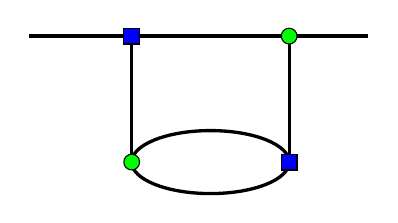
\begin{tikzpicture}  %G_3
            \draw[very thick] (0,4.3)--(4.3,4.3);
            \draw[very thick] (1.3,2.7)--(1.3,4.3);
            \draw[very thick] (3.3,2.7)--(3.3,4.3);
            \draw[very thick] (2.3,2.7)ellipse(1 and 0.4);
            \filldraw[fill=blue](1.2,4.2)rectangle(1.4,4.4);
            \filldraw[fill=green] (3.3,4.3)circle(0.1);
            \filldraw[fill=blue] (3.2,2.6)rectangle(3.4,2.8);
            \filldraw[fill=green] (1.3,2.7)circle(0.1);
        \end{tikzpicture}
        \captionsetup{justification=centering}
        \caption{Binary straddled signature $G_2$}
        \label{fig:g2}
\end{figure}

Now we introduce a new binary straddled signature $G_2$ as shown in Figure~\ref{fig:g2}. The signature matrix of 
$G_2$ is $
\left[\begin{smallmatrix}
w & b' \\ a' & c'
\end{smallmatrix}\right]$,
%\left[\begin{smallmatrix}1 + 2a^3 + b^3 & a^2 + 2ab^2 + bc^2 \\ a + 2a^2b + b^2c & a^3 + 2b^3 + c^3\end{smallmatrix}\right]$. We define 
where $w=1+ab$, $a'=a+b^2$, $b'=a^2+bc$ and $c'=ab+c^2$. Similar to $G_1$, we have
$\Delta' = \sqrt{(w-c')^2+4a'b'}$, two eigenvalues $\lambda'=\frac{-\Delta' + (w+c')}{2}$ and $\mu' = \frac{\Delta' + (w+c')}{2}$. If $a'\ne 0$, we have $x'=\frac{\Delta'-(w-c')}{2a'}$, $y'=\frac{\Delta'+(w-c')}{2a'}$ and if further $\Delta' \ne 0$ we can write its Jordan Normal Form as 
\begin{equation}\label{eqn:G2-JNF}
G_2 = \left(\begin{array}{ll}w & b' \\ a' & c'\end{array}\right)=\left(\begin{array}{cc}-x' & y' \\ 1 & 1\end{array}\right)\left(\begin{array}{ll}\lambda' & 0 \\ 0 & \mu'\end{array}\right)\left(\begin{array}{cc}-x' & y' \\ 1 & 1\end{array}\right)^{-1}.
\end{equation}


Similar to Proposition \ref{g1-rou}, we have the following claim on $G_2$.
 \begin{proposition} \label{c3}
If the signature matrix of $G_2$  is non-degenerate, then
 the ratio  $\lambda'/\mu'$ of its eigenvalues 
is not a root of unity \emph{unless} at least one of the following conditions holds, where 
$A = w + c', B = (c'-w)^2 + 4a'b'$.
% $A = 1+2ab+c^2$, $B=4a^3+4a^2b^2 + 4abc + 4b^3c + (c^2-1)^2$:
\begin{equation} \label{c3eq}\begin{cases}
A=0\\
B=0 \\
A^2+B=0\\
A^2+3B=0\\
3A^2 + B = 0\\
\end{cases}
\end{equation}
\end{proposition}



\begin{lemma} \label{y11x}
Suppose  $a,b,c \in \mathbb{Q}$, $a\neq0$ and $c\neq ab$ and $a,b,c$ do not satisfy any condition in  (\ref{c1eq}). Let $x=\frac{\Delta-(1-c)}{2 a}$,  $y=\frac{\Delta+(1-c)}{2 a}$ and $\Delta=\sqrt{(1-c)^2 + 4ab}$. Then 
for $\Holant ( \, [1,a,b,c] \, | =_3)$,
%problem $[1,a,b,c]$,\ 
\begin{enumerate}
    \item we can  interpolate $[y,1]$ on LHS;
    \item we can  interpolate $[1,x]$ on RHS except for 2 cases:
    %(by Remark under Lemma \ref{3.1.2}, the two cases happen when $y=-1$)
    %: 
    $[1,a,a,1]$, $[1,a,-1-2a, 2+3a]$.
\end{enumerate}  
\end{lemma}
\begin{proof}
This lemma follows from  Lemma \ref{3.1.1} and Lemma \ref{3.1.2}
using the binary straddled gadget $G_1$ with signature matrix $\left[\begin{smallmatrix}1 & b \\ a & c\end{smallmatrix}\right]$.  Note that $c\neq ab$ indicates that matrix $G_1$ is non-degenerate, and $\lambda/\mu$ not being a root of unity is equivalent to none of the equations in (\ref{c1eq}) holds.
\end{proof}

We have similar statements corresponding to $G_2$. When the signature matrix is non-degenerate and does not satisfy any condition in  (\ref{c3eq}), we can  interpolate the corresponding $[y',1]$ on LHS, and we can also interpolate the corresponding $[1,x']$ on RHS except when $y'=-1$.


\begin{definition} \label{d1}
For $\PlHolant ( \, [1,a,b,c] \, | =_3)$, with $a,b,c \in \mathbb{Q}$, $a \neq 0$, we say a binary straddled gadget $G$ \emph{works} if the signature matrix of $G$ is non-degenerate and the ratio of its two eigenvalues $\rlm$ is not a root of unity.
\end{definition}

\noindent
\begin{remark}
    
  Explicitly, the condition that $G_1$ \emph{works} is that $c \neq ab$ and $a,b,c$ do not satisfy any condition in (\ref{c1eq}), which is just the assumptions in Lemma \ref{y11x}. $G_1$ \emph{works} implies that it can be used to interpolate  $[y,1]$ on LHS, 
and to interpolate $[1,x]$ on RHS with two exceptions 
%($[1,a,a,1]$ and $[1,a,-1-2a, 2+3a]$)
for which we already proved the dichotomy. The $x,y$ are as stated in Lemma \ref{y11x}.

Similarly, when the binary straddled gadget $G_2$ \emph{works}, for the corresponding values $x'$ and $y'$,
we can  interpolate $[y',1]$ on LHS,
and we can interpolate  $[1,x']$ on RHS except when $y'=-1$.
 \end{remark}

\begin{figure}[ht] 
\centering
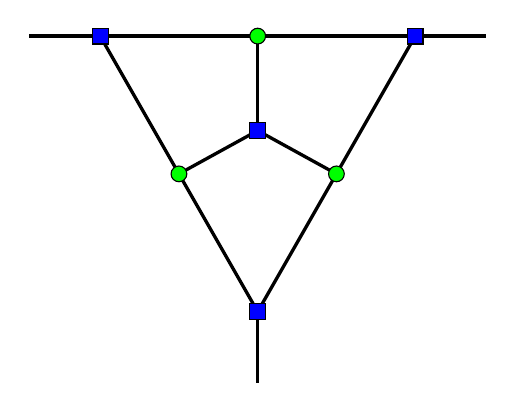
\begin{tikzpicture}  %G_4
\draw[very thick] (0.4,7.3)--(6.2,7.3);
\draw[very thick] (1.3,7.3)--(3.3,3.8);
\draw[very thick] (5.3,7.3)--(3.3, 3.8);
\draw[very thick] (3.3, 3.8)--(3.3, 2.9);
\draw[very thick] (3.3,6.1)--(3.3,7.3);
\draw[very thick] (3.3,6.1)--(4.3, 5.55);
\draw[very thick] (3.3,6.1)--(2.3,5.55);
\filldraw[fill=blue] (1.2,7.2) rectangle(1.4,7.4);  % 1.3  7.3
\filldraw[fill=blue] (5.2,7.2) rectangle(5.4,7.4);  % 5.3 7.3
\filldraw[fill=blue] (3.2,3.7) rectangle(3.4,3.9); % 3.3  3.8
\filldraw[fill=green] (3.3,7.3)circle(0.1);
\filldraw[fill=green] (4.3,5.55)circle(0.1);
\filldraw[fill=green] (2.3,5.55)circle(0.1);
\filldraw[fill=blue] (3.2, 6.0) rectangle(3.4, 6.2);     % 3.3, 6.1
\end{tikzpicture}
\captionsetup{justification=centering}
  \caption{A ternary gadget $G_3$}
  \label{f4}
\end{figure}

The ternary gadget $G_3$ in Figure \ref{f4} will be used in the proof here and later.


The unary signatures  $\Delta_{0}=[1,0]$ and $\Delta_{1}=[0,1]$
are called  the pinning signatures because they ``pin''
a variable to 0 or 1. Another useful unary signature is $\Delta_{2} = [1,1]$.
One good use of having unary signatures is that we can use Lemma~\ref{3.2} to get these three signatures. They 
are helpful as the following lemma shows.

\begin{lemma} \label{after-unary}
If $\Delta_{0}$, $\Delta_{1}$ and $\Delta_{2}$ can be interpolated on the RHS in
%the problem  
$\PlHolant ( \, [1,a,b,c] \, | =_3)$, 
where $a,b,c \in \mathbb{Q}$, $ab \neq 0$,
then  the problem is \numP-hard unless $[1,a,b,c]$ is affine or degenerate, in which cases it is in FP.
\end{lemma}
\begin{proof}
Connecting 
%unary signatures 
$[1,0]$, $[0,1]$ to $[1,a,b,c]$ on LHS respectively, we  get binary signatures $[1,a,b]$ and $[a,b,c]$. Then we can apply Corollary \ref{2-3},
and the problem is \numP-hard unless both $[1,a,b]$ and $[a,b,c]$ are in FP. When $ab\neq 0$, both $[1,a,b]$ and $[a,b,c]$ are in FP only when $[1,a,b,c]$ is (1) degenerate, i.e. $b=a^2$ and $c = a^3$, in which case the problem is in FP, (2) of the form $[1,a,1,a]$ which is resolved by Lemma~\ref{lemma:[1,a,1,a]} (when $a = \pm1$, $[1,a,1,a]$ is degenerate), (3) of the form $[1,a,a^2,a]$ which we will resolve later in this proof,  (4) $[1,a,b,c] = [1,1,1,-1]$ or $[1,-1,1,1]$ which we will resolve later in this proof, or (5) $[1,a,b,c] = [1,1,-1,-1]$ or $[1,-1,-1,1]$ which are affine and hence in FP.
% (3) $[1,a,b,c]=$  $[1,1,1-1]$ or $[1,-1,1,1]$ or $[1,-1,-1,-1]$ or $[1,1,-1,1]$ or $[1,1,-1,-1]$ or $[1,-1,-1,1]$, where the last two are affine and hence in FP. 

For case (2), if we connect $[1,1]$ to $[1,a,a^2,a]$, we get a binary signature $[1+a,a+a^2,a+a^2]$ which after normalization (when $a\neq -1$) is $[1,a,a]$. This problem is \numP-hard by Corollary~\ref{2-3} unless $a=\pm1$, in which cases the problem $[1,a,b,c]$ is $[1,1,1,1]$ or $[1,-1,1,-1]$ which are degenerate and thus in FP.


For case (3), due to the symmetry by flipping 0 and 1 in the  signature, it suffices to consider only $f= [1,1,1,-1]$ and $g=[1,-1,1,1]$; they   are neither affine nor degenerate. For both  $f$ and $g$ we use the gadget $G_3$ to produce  ternary signatures  $f' = [1,1,3,3]$
and $g' = [1,1,-1,3]$ respectively.  Neither are among  the exceptional cases above.
So $\Holant ( \, f \, | =_3)$ and $\Holant ( \, g\, | =_3)$ are both \numP-hard.
\end{proof}


\vspace{.1in}
%%%%%%%%%%%%%%%%%%%%%%%%%%%%%%%%%%%%%%%%%%%%%%%%%%%%%%%%

The following lemma lets us interpolate arbitrary unary signatures on RHS, in particular  $\Delta_{0}$, $\Delta_{1}$ and $\Delta_{2}$, from a binary gadget with a straddled signature and a suitable unary signature $s$ on RHS.  

\begin{lemma}[Vadhan, \cite{vadhan2001complexity}] \label{3.2}
Let $M\in \mathbb{R}^{2\times 2}$ be a non-singular signature matrix for a binary straddled gadget which is diagonalizable with distinct eigenvalues, and $s=[a,b]$ be a unary signature on RHS that is not a row eigenvector of $M$. Then $\{s\cdot M^j\}_{j\geq 0}$ can be used to interpolate any unary signature on RHS.
\end{lemma}



\subsection{Dichotomy for
$[1, a, b, c]$ when $ab\neq 0$ and $G_1$ works}  \label{large2}
\begin{figure}[h!] 
\centering
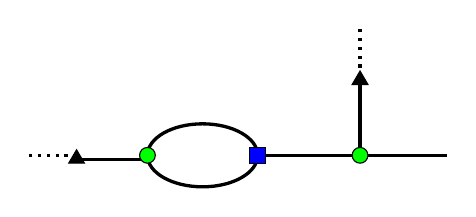
\begin{tikzpicture}  % nonli
\draw[very thick] (2,3.3)ellipse(0.7 and 0.4);
\filldraw[fill=black] (0.4,3.37)--(0.3,3.2)--(0.5,3.2)--cycle; 
\draw[very thick] (0.34,3.25)--(1.3,3.25);
\draw[very thick] (2.7,3.3)--(5.1,3.3);
\draw[very thick] (4,4.3)--(4,3.3);
\filldraw[fill=green] (1.3, 3.3)circle(0.1);  % 1.3 3.3
\filldraw[fill=blue] (2.6,3.2) rectangle(2.8,3.4);  % 2.7  3.3
\filldraw[fill=green] (4,3.3)circle(0.1);
\filldraw[fill=black] (4,4.37)--(3.9,4.2)--(4.1,4.2)--cycle;
\draw[very thick, dotted] (0.4,3.3) -- (-0.2,3.3);
\draw[very thick, dotted] (4, 4.3) -- (4,4.9);
\end{tikzpicture}
\captionsetup{justification=centering}
  \caption{Non-linearity gadget, where a triangle represents the unary gadget $[y,1]$}
  \label{non_li}
\end{figure}

Let us introduce a \emph{non-linearity} gadget in Figure \ref{non_li}. If we place in the non-linearity gadget the binary degenerate straddled signature $D$ on triangles (in the way that respects the bipartite structure), $f$ on squares and $(=_3)$ on circles, we get its signature
%If we follow the proof of the basic lemma in \cite{FanC21}, we can get a ternary RHS signature
 $[1,x] \otimes [1,x] \otimes [y^2+yb,ya+c]$.
% using a planar construction.
Note that it is a ternary planar gadget on RHS.
%This is obtained in the setting of
%$\plholant{[1,a,b,c]}{(=_3)}$.
The following two lemmas  will be used in the proof of  Theorem~\ref{g1works1}.



\begin{lemma} \label{1-1 X=1}
Let $a,b, c \in \mathbb{Q}$, $ab \neq 0$,  and
satisfy \\
\emph{(con1)} $a^3 - b^3 - ab(1-c) =0$ and\\
\emph{(con2)} $a^3+ab+2b^3=0$.\\
Then $\PlHolant ( \, [1,a,b,c] \, | =_3)$ is
\numP-hard unless it is $[1,-1,1,-1] = [1, -1]^{\otimes 3}$ which is degenerate, or a matchgate, in both cases the problem is in FP. 
\end{lemma}
\begin{proof}
If $a+b^2=0$  in addition to (\emph{con1}) and (\emph{con2})
with  $ab \neq 0$, then $[1,a,b,c] = [1,-1,1,-1]$ which is degenerate. Now we assume $a+b^2\ne0$. Here we use Gadget $G_2$. 

First assume $G_2$ \emph{works}. 
%By assumption $a+b^2\ne 0$,
Using  $a+b^2\ne 0$
together with (\emph{con1}) and  (\emph{con2}), we 
can verify that 
$\Delta = \sqrt{4(a+b^2)(a^2+bc)+(c^2-1)^2} \not =0$, and
%get $4(a+b^2)(a^2+bc) + (c^2-1)^2 \ne 0$, so 
we can write the Jordan Normal Form  $$G_2 = \left(\begin{array}{ll}1+ab & a^2+bc \\ a+b^2 & ab+c^2
\end{array}\right)=\left(\begin{array}{cc}-x & y \\ 1 & 1\end{array}\right)\left(\begin{array}{ll}\lambda & 0 \\ 0 & \mu\end{array}\right)\left(\begin{array}{cc}-x & y \\ 1 & 1\end{array}\right)^{-1},$$ where
%$\Delta = \sqrt{4(a+b^2)(a^2+bc)+(c^2-1)^2}$, 
$\lambda = \frac{1+2ab+c^2-\Delta}{2}$, $\mu = \frac{1+2ab+c^2+\Delta}{2}$, $x = \frac{\Delta+c^2-1}{2(a+b^2)}$, $y = \frac{\Delta-c^2+1}{2(a+b^2)}$. Because $G_2$ works, $[y,1]$ on LHS is  available. Use this $[y,1]$
in the non-linearity gadget in Figure \ref{non_li}, we get the unary signature $\left[y^{2}+y b, y a+c\right]$ on the RHS. By Lemma \ref{3.2}, we can interpolate any unary signature, in particular $\Delta_{0}$, $\Delta_{1}$ and $\Delta_{2}$ on RHS
and apply Lemma~\ref{after-unary}, unless $\left[y^{2}+y b, y a+c\right]$ is proportional to a row eigenvector of $G_3$, namely $[1,-y]$ and $[1, x]$. Thus the exceptions are $ya+c = x(y^{2}+y b)$ and $ya+c = -y(y^2+yb)$. Notice that now $xy = \frac{a^2+bc}{a+b^2}$. The first equation implies $c = ab$ or $a + b^2= 0$ or $a^3-b^3c+ab(-1+c^2) = 0$. The second equation implies $a+b^2=0$ or $f_1 =0$ where $f_1= a^3+4a^6+3a^5b^2+a^3b^3-c-4a^3c+6a^4bc-6a^2b^2c-b^3c-3a^2b^5c-3a^3c^2-3abc^2-4b^3c2-a^3b^3c^2-6ab^4c^2-4b^6c^2+3c^3+4a^3c^3+6a^2b^2c^3+3b^3c^3+a^3c^4+3abc^4+4b^3c^4-3c^5-b^3c^5+c^7$. So there are four exceptional cases, \begin{equation} \label {g3works} \begin{cases}
    c = ab \\
    a + b^2= 0\\
    a^3-b^3c+ab(-1+c^2) = 0\\
    f_1 = 0\\ \end{cases}
\end{equation}

 For each of them, together with (\emph{con1}) and (\emph{con2}), we get 3 equations and can solve them using
Mathematica\texttrademark{}.
For rational $a,b,c$, when $ab\neq0$, there are only two possible results --- $[1,-1,1,-1]$ and $[1,-\frac{1}{3}, -\frac{1}{3}, 1]$. The first one violates $a+b^2 \ne 0$, 
%Between them, the first is degenerate 
and the second is a matchgate and thus in $\operatorname{FP}$. For all other cases when $G_2$ works, we have
the pinnng signatures $\Delta_{0}$, $\Delta_{1}$  and $\Delta_{2}$
on the RHS and then the lemma is proved by Lemma \ref{after-unary}.

Now suppose $G_2$ does not work. Then by Proposition \ref{c3}, we get at least one more condition, either one in (\ref{c3eq}) or $(a+b^2)(a^2+bc) = (1+ab)(ab+c^2) $ which indicates that $G_2$ is degenerate. For each of the 6 conditions, together with (\emph{con1}) and (\emph{con2}), we can solve them using
Mathematica\texttrademark{} for rational $a,b,c$. The only 
solution is $[1,-1,1,-1]$ which  violates $a+b^2 \ne 0$.
%is degenerate. 
The proof of the  lemma is complete.
\end{proof}




\begin{lemma} \label{1-2 X=1}
Let $a,b, c \in \mathbb{Q}$, $ab \neq 0$,  and
satisfy\\
\emph{(con1)} $a^3 - b^3 - ab(1-c) =0$ and\\
\emph{(con2)}  $(a^4b+ab^4)^2 = (a^5+b^4)(b^5+a^4c)$.\\
Then $\PlHolant ( \, [1,a,b,c] \, | =_3)$ is
 \numP-hard unless it is $[1,a,a^2, a^3]$ which is degenerate, or a matchgate, in both cases the problem is in FP. 
\end{lemma}
\begin{proof}
Eliminating $c$ from  (\emph{con1}) and (\emph{con2})
we get 
 $a^{11}-a^9b+a^6b^4+a^5b^6-a^4b^5-a^3b^7+a^2b^9-b^{10}=0$, which, quite miraculously, can be factored as $(a^2-b) (a^9 + a^4 b^4 + a^3b^6 + b^9)=0$. If $b=a^2$, then with (\emph{con1}), we get $c=a^3$ thus the signature becomes $[1,a,a^2,a^3]$ which is degenerate. We  assume 
 % (\emph{con3}) 
 $a^9 + a^4b^4 + a^3b^6+b^9=0$, then the rest  of the
 proof is essentially the same as Lemma \ref{1-1 X=1}.
\end{proof}


\begin{theorem} \label{g1works1}
For $a,b, c \in \mathbb{Q}$, $ab \neq 0$, 
 if $G_1$ works, then $\PlHolant ( [1,a,b,c]  | =_3)$ is
 \numP-hard unless it is in the tractable cases of Theorem~\ref{thm:main} and thus in FP.
\end{theorem}


\begin{proof}
If $[1,a,b,c]$ has the form $[1,a,a,1]$ or $[1,a,-1-2a,2+3a]$
then the problem is in FP.  We now assume the signature is not of these two forms.
By Lemma \ref{y11x}, when $G_1$ works, we can interpolate $[y,1]$ on LHS and also  $[1,x]$ on RHS.



Let us write down the Jordan Normal Form again: $$G_1 = \left(\begin{array}{ll}1 & b \\ a & c\end{array}\right)=\left(\begin{array}{cc}-x & y \\ 1 & 1\end{array}\right)\left(\begin{array}{ll}\lambda & 0 \\ 0 & \mu\end{array}\right)\left(\begin{array}{cc}-x & y \\ 1 & 1\end{array}\right)^{-1},$$  $\lambda=\frac{-\Delta+(1+c)}{2}$, $\mu=\frac{\Delta+(1+c)}{2}$, $x=\frac{\Delta-(1-c)}{2 a}$,  $y=\frac{\Delta+(1-c)}{2 a}$, $\Delta=\sqrt{(1-c)^2 + 4ab}$.

Using $[y,1]$ and the gadget in Figure \ref{non_li}, we get  $\left[y^{2}+y b, y a+c\right]$ on the RHS.
We can interpolate  $\Delta_{0}$, $\Delta_{1}$ and $\Delta_{2}$ on RHS unless $\left[y^{2}+y b, y a+c\right]$ is proportional to a row eigenvector of $G_1$, namely $[1,-y]$ or $[1, x]$, according to Lemma \ref{3.2}. Thus the exceptions are $y a+c = (y^{2}+y b)x$ or $y a+c = -y(y^{2}+y b)$. The first equation implies $a^{3}-b^{3}-a b(1-c)=0$ or $c=ab$. The second equation implies $c=ab$ or $c=1+a-b$. 

By assumption  $G_1$ works, so $c\ne ab$. Thus, we consider two exceptional cases.


\noindent 
\textbf{Case 1}: $a^{3}-b^{3}-a b(1-c)=0$

In this case, we have $1-c = \frac{a^3-b^3}{ab}$ and thus $\Delta = \sqrt{(1-c)^2+4ab} = |\frac{a^3+b^3}{ab}|$.  One condition ($4ab + c^2 - 2c+1 = 0$) in (\ref{c1eq}) is the same as $\Delta=0$.  Since $G_1$ works, we have $\Delta \neq 0$ and thus $a^3+b^3\neq 0$, which is equivalent to $a+b\ne 0$ when $a,b\in \mathbb{Q}$.


%\noindent
\begin{description}
    \item{Subcase 1: $ \frac{a^3+b^3}{ab} > 0$.}
%\textbf{Subcase 1:} 
%
 We have  $[1,x] = [1,\frac{\Delta - \left(1-c\right)}{2a}] = [1, \frac{b^2}{a^2}]$ on RHS. Connect $[1,x]$ to $[1,a,b,c]$ on LHS, we get the binary signature $[1+\frac{b^2}{a}, a+\frac{b^3}{a^2}, b+\frac{b^2c}{a^2}]$ on LHS. Note that $a+\frac{b^3}{a^2} \neq 0$ when $a+b \neq 0$.
%
%We have $a+\frac{b^3}{a^2}\neq 0$. 
%The problem $[1+\frac{b^2}{a}, a+\frac{b^3}{a^2}, b+\frac{b^2c}{a^2}]$ 
It is \numP-hard (and thus the problem $[1,a,b,c]$ is \numP-hard) unless one of the tractable conditions in Corollary~\ref{2-3} holds. It turns out that the only possibilities are either (1) 
first case in Corollary \ref{2-3}, i.e. $(1+\frac{b^2}{a})(b+\frac{b^2c}{a^2}) = (a+\frac{b^3}{a^2})^2$, which becomes $\left(a^2-b \right)\left(a^3+ab+2b^3 \right) = 0$ after substituting $c = \frac{ab-a^3+b^3}{ab}$,
%To quickly verify, one might first plug c into b+\frac{b^2c}{a^2} to get \frac{b^2(a+b^2){a^3}}
or (2) the second and third case in Corollary \ref{2-3}, which implies $(a = -b^2) \wedge (c= - b^3)$ and thus the problem $[1,a,b,c]$ becomes the problem $[1,-b^2,b,-b^3]$,
% To verify this, a quick way is to first plug c into b+\frac{b^2c}{a^2} to get \frac{b^2(a+b^2){a^3}}, and then set the ratio between \frac{b^2(a+b^2){a^3}} and 1+\frac{b^2}{a} to be -1
or (3) the fourth case in Corollary~\ref{2-3},
%$1+\frac{b^2}{a} = b+\frac{b^2c}{a^2}$, which 
which implies $(a=b) \wedge (c=1)$ or $(a = -b^2) \wedge (c= - b^3)$, where in the former case $[1,a,b,c]$ is of the matchgate form $[1,a,a,1]$ and thus in FP. 

We now deal with the case (1).
When $a^2-b = 0$, together with $a^3-b^3=ab\left(1-c\right)$, we have $c = a^3$, and thus $[1,a,b,c]$ is degenerate. When $a^3+ab+2b^3 = 0$, together with $a^3-b^3=ab\left(1-c\right)$, by Lemma \ref{1-1 X=1}, $[1,a,b,c]$ is \numP-hard (with $a+b\ne0$ ruling out the exception). 

We now deal with the case $[1,-b^2,b,-b^3]$. If $b=0, \pm 1$, it is degenerate or affine. Now assume $b\neq 0, \pm 1$. $G_1 = \smm{1}{b}{-b^2}{b^3} = \smmv{1}{-b^2}\cdot\smmh{1}{b}$. Then we can get $[1,-b^2]$ on the  LHS.
Note that connecting three copies of $[1,b]$ with $[1,-b^2,b,-b^3]$ on LHS produces a global factor 
$1-b^6 \ne 0$.  Connect $[1,-b^2]$ twice to $[1,0,0,1]$ on RHS, and we get $[1,b^4]$ on RHS. Connect $[1,b^4]$ back to $[1,-b^2, b, -b^3]$ on LHS, and we get a binary signature $g=[1-b^6, -b^2 + b^5, b-b^7]$, which by Corollary \ref{2-3} is \numP-hard unless $b = \pm1$ which has been discussed, and therefore $[1,-b^2, b, -b^3]$ is also \numP-hard. 


 \item{Subcase 2: $\frac{a^3+b^3}{ab} < 0$}. We have $[y,1] = [-\frac{b^2}{a^2},1]$ on LHS. Connecting two copies of $[y,1]$ to $(=_3)$ we get $[y^2, 1] = [\frac{b^4}{a^4}, 1]$ on RHS.
 Connecting it back to LHS, we  get a binary signature $[\frac{b^4}{a^4}+a,\frac{b^4}{a^3}+b,\frac{b^5}{a^4}+c]$ on LHS. 
It is \numP-hard  unless one of the tractable conditions in Corollary~\ref{2-3} holds. It turns out that the only possibilities are either
 $(a^4b+ab^4)^2 = (a^5+b^4)(b^5+a^4c)$, or $(a=b) \wedge (c=1)$ which is the matchgate case and thus in FP. We now deal with the former case. Together with $a^3-b^3=ab\left(1-c\right)$, by Lemma \ref{1-2 X=1}, $[1,a,b,c]$ is \numP-hard unless it is degenerate.
\end{description}

\noindent 
\textbf{Case 2}: $1+a-b-c=0$


In this case, $\Delta=|a+b|$, and since
$G_1$ works, one condition is $4ab+c^2-2c+1=0$ in (\ref{c1eq})
which says $\Delta \ne 0$,  and thus $a+b \neq 0$.

If $a+b > 0$, then 
$\Delta=a+b$, and $x = \frac{a+b-(1-c)}{2a} = 1$. Then we can interpolate $[1,x] = [1,1]$ on RHS (as $y = \frac{a+b+(1-c)}{2a} = \frac{b}{a}\ne -1$). Else,  $a+b < 0$,  then 
$\Delta=-(a+b)$, and $y = \frac{-a-b + (1-c)}{2a} = \frac{-a-b + (b-a)}{2a}= -1$. We can  get $[1,1]$ on RHS by connecting two copies of $[y,1]=[-1,1]$ to $[1,0,0,1]$. Then connecting $[1,1]$ to $[1,a,b,c]$ on LHS we get a binary signature $[a+1,a+b, a+c]$ on LHS. Again we can apply
 Corollary \ref{2-3} to it, and conclude that it is
 \numP-hard. It turns out that  
 the only feasible cases of tractability leads to 
  $[1,a,-1-2a,2+3a]$, and $(c=1)\wedge(a=b)$, in both cases the problem is in FP.
%  for which we have a dichotomy
% Lemma~\ref{p3}.
 %%% X=1 gives (a+b = \pm (a+1). but (+) ==> b=1,c=a is
 %%% [1,a,1,a] violates  c \not =ab.
% For all other cases it is 
% \numP-hard, and  
This proves the \numP-hardness of
$\Holant ( \, [1,a,b,c] \, | =_3)$.
%
%
% \noindent\textbf{Otherwise,} $\Delta=-a-b>0$. $y = \frac{-a-b + (1-c)}{2a} = \frac{-a-b + (b-a)}{2a}= -1$. The unary signature that can be interpolated on LHS is $[y,1] = [-1,1]$. We connect two copies of $[-1,1]$ to $[1,0,0,1]$ on RHS to get a unary $[1,1]$ on RHS. Then connect $[1,1]$ to $[1,a,b,1+a-b]$ on LHS and we will get a binary signature $[1+a,a+b,1+a]$ on LHS. Then the proof is same as the case $\Delta=b+a > 0$.
%
%So now we've proved Theorem \ref{g1works1}.
%
\end{proof}


\subsection{Dichotomy for $[1,a,b,0]$}   \label{large3}



\begin{theorem}   \label{1ab0}
The problem  $[1,a,b,0]$ 
for $a,b \in \mathbb{Q}$ is
 \numP-hard
 unless it is in the tractable cases of Theorem~\ref{thm:main} and thus in FP.
\end{theorem}

\begin{proof}
If $ab\neq 0$ and $G_1$ works, then this is proved in
Theorem~\ref{g1works1}.
 If $a=b=0$, it is degenerate and in FP. We divide the rest into three cases: \begin{enumerate}
    \item $ab\neq 0$ and $G_1$ does not work;
    \item $f = [1,a,0,0]$ with $a\neq 0$;
    \item $f= [1,0,b,0]$ with $b\neq 0$.
\end{enumerate}

\noindent 
$\bullet$ Case 1:  $ab\neq 0$ in $f = [1,a,b,0]$ and $G_1$ does not work. Since $c=0 \ne ab$, this implies that at least one equation in (\ref{c1eq})
holds. After a simple derivation, we  have the following family of signatures to consider:   $[1,a,-\frac{1}{ka}, 0]$, for $k = 1, 2, 3, 4$. %$[1,a,-\frac{1}{3a}, 0]$ and $[1,a,-\frac{1}{4a}, 0]$.

We  use $G_3$ to produce another symmetric ternary signature in each case. If the new signature is \numP-hard, then so is the given signature. We will describe the case $[1,a,-\frac{1}{a}, 0]$ in more detail; the other three types ($ k=2, 3, 4$) are similar.

For $k=1$, the gadget $G_3$ produces $g= [3 a^3+4, a^4-a-\frac{2}{a^2}, -a^2+\frac{1}{a}+\frac{1}{a^4}, a^3+3]$. %with $[1,a,-\frac{1}{a}, 0]$. 
For $a= -1$, this is $[1,0,-1,2]$, which has the form $[1,a',-1-2a', 2+3a']$ and is in FP. Below we assume $a \not = -1$. Then all entries of $g$ are nonzero.

We claim that the gadget $G_1$ works using $g$. Since $a\in \mathbb{Q}$, it can be checked that $g$ is non-degenerate since $(a^4-a-\frac{2}{a^2})( -a^2+\frac{1}{a}+\frac{1}{a^4}) = (3a^3 + 4)(a^3 + 3)$ has no solution, and that no equation in (\ref{c1eq}) has a solution applied to $g$. Hence, $G_1$ works using $g$ and we may apply Theorem \ref{g1works1} to $g$. Using the fact that $a\in\mathbb{Q}$, one can show that $g$ cannot be a Gen-Eq because it has no zero entry, nor can it be affine or degenerate. Also, it can be checked that there is no solution for $a$ if we were to impose the condition that $g$ is a matchgate, i.e. $(3 a^3+4 = a^3+3) \wedge (a^4-a-\frac{2}{a^2} = -a^2+\frac{1}{a}+\frac{1}{a^4})$, and also $ a = -1$ is the only solution for $g$ being in the form $[1,a',-1-2a',2+3a']$. Thus $[1,a,-\frac{1}{a}, 0]$ is \numP-hard.

\noindent 
$\bullet$ Case 2: $f= [1,a,0,0]$ with $a\neq 0$. 
The gadget $G_3$ produces $g'=[3a^3+1, a^4+a, a^2, a^3]$. Since $a\in \mathbb{Q}$, $3a^3+1\neq0$. 
%
If $a=-1$, $g'=[-2, 0,1,-1]$ and 
% MK13
it suffices to consider $[1,-1,0,2]$ (which is $-1$ times the reversal $[-1,1,0,-2]$ 
obtained by swapping and roles of 0 and 1), in which case $G_2$ works where the matrix $G_2=\left[\begin{smallmatrix}1 & 1 \\ -1 & 4\end{smallmatrix}\right]$. We can interpolate $[1,x] = [1, -\frac{3 + \sqrt{5}}{2}]$ on RHS. Connect it back to $[1,-1,0,2]$ and get a binary signature $[\frac{5+\sqrt{5}}{2}, -1, -(3+\sqrt{5})]$ on LHS, which, by Corollary \ref{2-3}, is \numP-hard. Thus, $[1,-1, 0,2]$ is \numP-hard and so is $[1,a,0,0]$.

Else, $a\neq -1$.
%, since also we assumed  $a\neq0$, 
%we have $a^4+a\neq0$, $a^2 \neq 0$. 
We claim that the gadget $G_1$ works using $g'$.
The signature $g'$ is non-degenerate 
since $a\in \mathbb{Q}$  is nonzero
and thus  $(a^4+a)a^2 \not =(3a^3+1)a^3$.
Also 
 no equation in (\ref{c1eq}) has a solution applied to $g'$. Hence, $G_1$ works using $g'$ and we may apply Theorem \ref{g1works1} to $g'$. Using the fact that $a\in\mathbb{Q}$, one can show that $g'$ cannot be a Gen-Eq because it has no zero entry, nor can it be affine or degenerate. Also, there is no solution for $g'$ being a matchgate or in the form $[1,a',-1-2a',2+3a']$. Thus $[1,a,0, 0]$ is \numP-hard.

%To conclude, $[1,a,0,0]$ with $a\neq 0$ is  \numP-hard.

\noindent 
$\bullet$ Case 3: 
 $f = [1,0,b,0]$ with $b\neq 0$. The gadget $G_1$ produces a binary straddled signature $G_1=\left[\begin{smallmatrix}1 & b \\ 0 & 0\end{smallmatrix}\right] = \left[\begin{smallmatrix} 1 \\ 0 \end{smallmatrix}\right]\cdot \left[\begin{smallmatrix}1 & b \end{smallmatrix}\right]$ 
which decomposes into 
a unary signature $[1,b]$ on RHS and 
a unary signature $[1, 0]$ on LHS.
This gives us a reduction
$\PlHolant ( [1,b^2,b] | ( =_3)) \le_T
\PlHolant ( \, f \, | =_3)$ by the P3EM argument. The problem 
$\PlHolant ( [1,b^2, b]  | =_3)$ is \numP-hard except $b =\pm 1$,
by Corollary \ref{2-3}, which implies that $\PlHolant ( \, f \, | =_3)$ is also \numP-hard
when $b \ne \pm 1$. If $b = \pm 1$,
then $f$ is affine, and $\PlHolant ( \, f \, | =_3)$ is in FP.
%
 %We can split it and get $[1,b]$ on RHS (since for each 3 redundant $[1,0]$ on LHS, connect them to $(=_3)$ on RHS and we get a global factor \textbf{1}). Next connect $[1,b]$ to 
 %$[1,0,b,0]$ and we get binary signature $[1,b^2, b]$ on LHS. By Theorem \ref{2-3}, unless $b=\pm 1$, it is \numP-hard and so is the given signature. When $b=\pm 1$, this is $[1,0,1,0]$ or $[1,0,-1,0]$, both of which are in the affine class and so are in FP.
%
%So $[1,0,b,0]$ is \numP-hard unless $b=\pm1$, which is in FP.
%
\end{proof}


\subsection{Dichotomy for $[1,a,0,c]$}  \label{large4}
\begin{theorem} \label{1a0c}
The problem $[1,a,0,c]$ with $a,c\in \mathbb{Q}$ is \numP-hard unless $a=0$, in which case it is Gen-Eq and thus in FP.
\end{theorem}
\begin{proof}
When $a=0$, it is Gen-Eq and so is in FP. When $a\neq 0$, if $c=0$, it is \numP-hard by Theorem \ref{1ab0}. In the following we discuss $[1,a,0,c]$ with $ac\neq 0$.

 If $c=\pm1$, the signature is $[1,a,0,1]$ or $[1,a,0,-1]$. We use $G_2$ to produce a ternary signature $g=[3a^3+1, a^4+a, a^2, a^3 + 1]$ (both mapped to the same signature, surprisingly). If $a=-1$, it is $[1,0,-\frac{1}{2}, 0]$ after normalization, which by Theorem \ref{1ab0} is \numP-hard and so is the given signature $[1,-1,0,1]$. If $a\neq -1$, then $g$ has no zero entry. We then claim that the gadget $G_1$ works using $g$. It can be checked that $g$ is non-degenerate since $(a^4+a)a^2=(3a^3+1)(a^3+1)$ has no solution, and that no equation in (\ref{c1eq}) has a solution applied to $g$. Hence, $G_1$ works using $g$ and we may apply Theorem \ref{g1works1} to $g$. Using the fact that $a\in\mathbb{Q}$, one can show that $g$ cannot be a Gen-Eq because it has no zero entry, nor can it be affine or degenerate.  Also, it can be checked that the only solution for $a$ if we were to impose
 the condition that $g$ is a matchgate or in the form $[1,a',-1-2a',2+3a']$ for some $a'$ is $a=0$. Thus $[1,a,0,\pm 1]$ are both \numP-hard.


%%%%%%%%

Now assume $c \ne 0, \pm 1$. We claim that the gadget $G_1$ works. It can be checked that for the non-degenerate matrix $G_1=\smm{1}{0}{a}{c}$, $\Delta = |1-c|$, $\rlm \in \{c, \frac{1}{c}\}$  is not a root of unity. 
Next we claim that we can obtain $[1,0]$ on RHS.
If $c<1$ by Lemma~\ref{y11x}
we can interpolate $[1,x]=[1,0]$  on RHS 
%by the Remark on Definition \ref{d1} 
with two exceptions to which we already give a dichotomy (see
the Remark after Definition \ref{d1}). 
If $c>1$,  we can interpolate $[y,1] = [0,1]$ on LHS and so the gadget in Figure \ref{non_li} produces  $[0,c]$ on RHS, which is not
proportional to the 
 row eigenvectors $[1,-y] = [1,0]$ and 
 $[1,x] = [1,\frac{c-1}{a}]$ of  $G_1$. 
 By Lemma \ref{3.2}, we can interpolate any unary gadget on RHS, including $[1,0]$. Thus we can always get $[1,0]$ on RHS. Connect $[1,0]$ to $[1,a,0,c]$  and we will get a binary signature $[1,a,0]$ on LHS, which is \numP-hard by Corollary \ref{2-3}. Therefore $[1,a,0,c]$ is \numP-hard when $c\ne 0, \pm 1$. 
\end{proof}


\subsection{Dichotomy for $[1,a,b,c]$ when $abc\ne0$}

We need three lemmas to handle some special cases. Lemma~\ref{p1} is a part of Theorem~\ref{g1works1} 
(one verifies that $G_1$ works, in fact for $[1,-b^2, b, -b^3]$ the condition  (\ref{c1eq}) amounts to $b=1$, and the $b=0$ case is degenerate thus trivially in FP). For convenience,
we state it explicitly here.



\begin{lemma} \label{p1}
The problem $[1,-b^2, b, -b^3]$ with $b\in \mathbb{Q}$ is \numP-hard unless $b=0, \pm 1$, which is in FP.
\end{lemma}

The next lemma is not part of Theorem~\ref{g1works1}  since the condition  (\ref{c1eq}) fails for 
$[1, a, -\frac{1}{a}, -1]$.

\begin{lemma} \label{p2}
The problem $[1, a, -\frac{1}{a}, -1]$ with $a\in \mathbb{Q}$, $a\neq 0$ is \numP-hard unless $a=\pm 1$, in which case it is in FP.
\end{lemma}
\begin{proof}
If $a=\pm 1$, $[1,1,-1-1]$ is   affine and $[1,-1,1,-1]$ is degenerate, both of which are in FP. Now we assume $a\neq \pm 1$ (so the matrix $\smm{a^{-2}}{a}{1}{1}$ is invertible). We use the ternary gadget $G_3$ to get the signature $g = [3a^3+\frac{1}{a^3}+4, a^4-\frac{1}{a^2},-a^2+\frac{1}{a^4},a^3+\frac{3}{a^3}+4]$ on LHS. A direct computation (using Mathematica) shows that $G_1$ always works for $g$ unless $ a = -1$. Therefore, by Theorem~\ref{g1works1} we have $g$ is \numP-hard and then $[1,a,-\frac{1}{a},-1]$ is \numP-hard unless $g$ is in the tractable cases in Theorem~\ref{thm:main}. The only solution for $g$ being in the tractable cases in Theorem~\ref{thm:main} is $a = \pm1$. This completes our proof.
\end{proof}


\begin{lemma} \label{c=ab}
The problem $[1,a,b,ab]$ with $a,b\in \mathbb{Q}$ and $a,b\ne 0$ is \numP-hard unless it is degenerate or  affine, which is in FP.
\end{lemma}
\begin{proof}
\begin{figure}[h!] 
    \centering
    \begin{subfigure}[b]{0.3\textwidth}
        \centering
        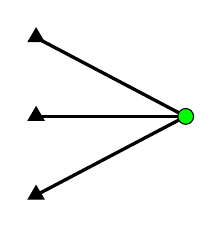
\begin{tikzpicture}  % i1
            \draw[very thick] (0.3,5.05) -- (2.2,4.05);
            \draw[very thick] (0.3,4.05) -- (2.2,4.05);
            \draw[very thick] (0.3,3.05) -- (2.2,4.05);
            \filldraw[fill=black] (0.3,5.17)--(0.2,5)--(0.4,5)--cycle;
            \filldraw[fill=black] (0.3,4.17)--(0.2,4)--(0.4,4)--cycle;
            \filldraw[fill=black] (0.3,3.17)--(0.2,3)--(0.4,3)--cycle;
            \filldraw[fill=green] (2.2, 4.05)circle(0.1);

        \end{tikzpicture}
        %\caption{$i1$}
                 \captionsetup{justification=centering}
  \caption{}
        \label{i1}
    \end{subfigure}
    \begin{subfigure}[b]{0.3\textwidth}
        \centering
        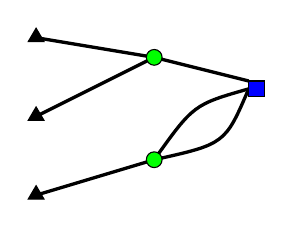
\begin{tikzpicture}  % i2
           \draw[very thick] (0.3,5.05)--(1.8,4.8);
        \draw[very thick] (0.3,4.05)--(1.8,4.8);
        \draw[very thick] (0.3,3.05)--(1.8,3.5);
        \draw[very thick] (1.8,4.8) -- (3,4.5);
        \draw[very thick] (1.8,3.5).. controls (2.3, 4.2) ..(3,4.4);
        \draw[very thick] (1.8,3.5) .. controls (2.7, 3.7)..(3,4.4);
        \filldraw[fill=black] (0.3,5.17)--(0.2,5)--(0.4,5)--cycle;
        \filldraw[fill=black] (0.3,4.17)--(0.2,4)--(0.4,4)--cycle;
        \filldraw[fill=black] (0.3,3.17)--(0.2,3)--(0.4,3)--cycle;
        \filldraw[fill=green] (1.8,4.8) circle (0.1);
        \filldraw[fill=green] (1.8,3.5) circle (0.1);
        \filldraw[fill=blue] (3,4.3)rectangle(3.2,4.5);

        \end{tikzpicture}
                \captionsetup{justification=centering}
  \caption{}
        %\caption{$i2$}
        \label{i2}
    \end{subfigure}
    \captionsetup{justification=centering}
    \caption{Two gadgets where each triangle represents the unary gadget $[1,a]$}
    \label{2g41a}
\end{figure}

If $a=-1$ and $b= \pm 1$
then  problem is in FP. Indeed,  $[1,-1,1,-1]$ is degenerate, and  $[1,-1,-1,1]$ can be transformed to matchgate;
both problems are  in FP. We therefore now assume it is not the case that both $a=-1$ and $b= \pm 1$.

We first use $G_3$ to construct a ternary signature $h = [-b^4+3b^2-2, b^4-2b^3-b^2+2b, 2b^3-b^2-2b+1, -2b^4+3b^2-1]$ on LHS, which can be normalized to $h = [2-b^2,b^2-2b,2b-1,1-2b^2]$ after dividing $(b+1)(b-1)$. 
Using gadget $G_1$, we have a degenerate matrix   $G_1 = \smm{1}{b}{a}{ab} =  \smmv{1}{a}\cdot \smmh{1}{b}$. We  get $[1,b]$ on RHS if $[1,a]$ can appropriately form some nonzero global factor.

Figure \ref{2g41a} indicates two different ways of ``absorbing'' $[1,a]$ on LHS. Importantly, we place 
$g$ instead of $[1,a,b,ab]$ on the square vertex.  Figure~\ref{i1} provides a factor $1+a^3$ which is nonzero if $a \neq -1$. When $a = -1$,  Figure~\ref{i2} provides a factor $2b^2-4b+2 = 2(b-1)^2$ which is nonzero unless $b=1$. Therefore, we can interpolate $[1,b]$ on RHS. Connect $[1,b]$ back to $[1,a,b,ab]$ on LHS and we get the binary signature $g=[1+ab, a+b^2, b+ab^2]$. If $a + b^2 = 0$, the given signature is $[1, -b^2, b, -b^3]$ which, according to Lemma \ref{p1}, is \numP-hard (the exceptions in Lemma \ref{p1} do not apply as $b \ne 0$ and if $b = \pm 1$ then $a =-b^2 = -1$ which is excluded.)
%as
%we assumed just now, it is not $[1,-1,\pm 1,\mp 1]$). 
Now we assume $a+b^2 \neq 0$. Normalize $g$ by dividing $a+b^2$, we have the binary signature $[\frac{1+ab}{a+b^2},1,\frac{b+ab^2)}{a+b^2}]$ on LHS. 
Applying Corollary \ref{2-3} to $g$, it is \numP-hard (and so is the given signature $[1,a,b,ab]$) unless \begin{enumerate}
    \item $(1+ab)(b+ab^2) = (a+b^2)^2$. This implies $\left(a^2-b \right)\left(b^3-1 \right)=0$. If $a^2-b=0$, the given signature is $[1,a,a^2,a^3]$ and  is degenerate. If $b^3-1=0$, since $b\in\mathbb{Q}$, we have $b=1$ and  $a
    \ne  -b^2 = -1$, and the given signature is $[1,a,1,a]$. This is resolved by Lemma~\ref{lemma:[1,a,1,a]}.
    \item $\frac{1+ab}{a+b^2} = 1$ and $\frac{b+ab^2}{a+b^2}=-1$. 
    Dividing the two expressions gives $b=-1$. This implies $a=0$ 
    and therefore violates our assumption that $a \neq 0$.
    %%% excellent!
    % To see this, note that b+ab^2 = b(1+ab).
    \item $\frac{1+ab}{a+b^2} = -1$ and $\frac{b+ab^2}{a+b^2}= 1$. No $(a,b)$ pair solves these two equations, under the assumption $a +b^2 \ne 0$.
    %%%1+ab = -(a+b^2) = -(b+ab^2)
    %% 1-b = ab(b-1)
    %a(1-b^2)+b(b-1)=0
    %b=1 or a+ab+b=0
    %b=1-> 1+a = -(1+a) so a=-1 excluded.
    % so a+ab+b=0
    % subs to 1) 1-a-b = -a-b^2
    % b^2 -b+1=0 not rational.
    %
%%%%%%%%
    %Hi professor, I just replied your e-mail about the line 990 quesiton, ok will look.
    \item $\frac{1+ab}{a+b^2} = \frac{b+ab^2}{a+b^2}$. We have either $b=1$ or $ab=-1$. If $b = 1$, then $[1,a,b,ab]$ becomes $[1,a,1,a]$ which is \numP-hard by Lemma~\ref{lemma:[1,a,1,a]} unless $a = 0$ (this violates our assumption) or $a= \pm 1$, in which cases the signature is affine and therefore the problem is in FP. If $ab=-1$, then  $[1,a,b,ab]$ becomes $[1,a,-\frac{1}{a},-1]$ which is \numP-hard by Lemma~\ref{p2} unless $a=\pm1$, in which cases the signature is affine and therefore the problem is in FP.
    \end{enumerate}
Note that since $a,b\ne 0$, $[1,a,b,ab]$ cannot be Gen-Eq. The lemma is  proved.
%the above sentence is also not necessary.
\end{proof}

Now we prove
%
% Till now, we already proved the dichotomy for $ab\neq 0$ and $G_1$ works, dichotomy for $[1,a,b,c]$ with $abc=0$ (problem $[1,0,b,c]$ with $bc\neq0$ can be taken care of by normalizing and flipping 0 and 1 and get the form $[1,a,0,c]$ with $ac\neq 0$). To problem $[1,a,b,c]$, the remaining part is only the case when $G_1$ does not work and $abc\neq 0$. We present the next main Theorem of our work:
\begin{theorem} \label{large5}
The problem $[1,a,b,c]$ with $a,b,c \in \mathbb{Q}$, $abc\ne0$, is \numP-hard unless it is in the tractable cases in Theorem~\ref{thm:main}.
\end{theorem}
\begin{proof}
 By Proposition~\ref{g1-rou}, Theorem \ref{g1works1} and Lemma \ref{c=ab} it suffices to consider the case when the ratio of two eigenvalues in $G_1=\smm{1}{b}{a}{c}$ is a root of unity and $c \neq ab$. If the ratio of eigenvalues of $G_1$ is a root of unity, we know at least one condition in (\ref{c1eq}) holds. For  convenience, we list the conditions in (\ref{c1eq}) here and label them as $R_i$ where $i=1,2,3,4,5$:
\begin{equation} \label{j1}
    R = \bigvee_{i=1}^{5} R_i,
    %R_1\vee R_2 \vee R_3 \vee R_4 \vee R_5 
    \ \ \text{where} \begin{cases}
     R_1: c=-1\\
     R_2: ab + c^2+c+1=0\\
     R_3: 2ab+c^2+1=0\\
     R_4: 3ab+c^2-c+1=0\\
     R_5: 4ab+c^2-2c+1=0\\
    \end{cases}
\end{equation}

% If $G_1$ \emph{works} then the theorem follows from 
% Theorem \ref{g1works1}.  When $c=ab$, it follows from Lemma \ref{c=ab}.
%$[1,a,b,c]$ for $a,b,c\ne 0$ has a dichotomy when the gadget $G_1$ works by Theorem \ref{g1works1}. 
% Recall that $G_1$ does not work iff either the matrix $G_1=\smm{1}{b}{a}{c}$ is degenerate (i.e., $c=ab$) or the ratio of its two eigenvalues is a root of unity (i.e., any one condition in (\ref{c1eq})). So below we assume that $c\ne ab$ and at least one condition in (\ref{c1eq}) holds. 

We apply $G_{3}$ on $[1,a,b,c]$, i.e.\ placing squares to be $[1,a,b,c]$ and circles to be $=_3$, to produce a ternary signature $[w,x,y,z]=[1+3a^3+3a^2b^2+b^3c, a+a^4+2a^2b+a^2bc+2ab^3+b^2c^2, a^2+ab^2+2a^3b+b^4+2ab^2c+bc^3, a^3+3a^2b^2+3b^3c+c^4]$. If $w \neq 0$ and $G_1$ works on $[w,x,y,z]$, by Theorem \ref{g1works1} we have $[w,x,y,z]$ is \numP-hard and thus $[1,a,b,c]$ is \numP-hard unless at least one condition $S_i$ listed below holds, where $i=1,2,3,4,5,6,7$:
\begin{equation} \label{j2}
    S = \bigvee_{i=1}^{7} S_i
    %S_1 \vee S_2 \vee S_3 \vee S_4 \vee S_5 \vee S_6 
    \ \ \text{where} \begin{cases}
    S_1 : x^2=wy \wedge y^2=xz\ (\text{degenerate form})\\
    S_2 : x=0 \wedge y=0\ (\text{Gen-Eq form})\\
    S_3 : w=y \wedge x=0 \wedge z=0\ (\text{affine form $[1,0,1,0]$}) \\
    S_4 : w+y=0 \wedge x = 0 \wedge z=0\ (\text{affine form $[1,0,-1,0]$})\\
    S_5: w = z \wedge x = y\ (\text{matchgate-realizable form $[a',b',b',a']$}) \\
    S_6: w = -z \wedge x = -y\ (\text{matchgate-realizable form $[a',b',-b',-a']$}) \\
    S_7: -w-2x = y \wedge 2w + 3x = z\ (\text{form $[3a'+b',-a'-b',-a'+b',3a'-b']$})
    \end{cases}
\end{equation} 
\noindent Note that the affine forms $[1,1,-1,-1]$ and $[1,-1,-1,1]$ are special forms of  $[a,b,b,a]$ and  $[a,b,-b,-a]$. Solve the equation system $R \wedge S$ for variables $a,b,c \in \mathbb{Q}$, we have the following solutions:
\begin{itemize}
    \item $a=c=-1, b=1$; the problem $[1,-1,1,-1]$ is in FP since it is degenerate;
    \item $a=1, b=c=-1$; the  problem $[1,1,-1,-1]$ is in FP since it is affine;
    % \item $a=-1, b=c=1$; the problem $[1,-1,1,1]$ is \numP-hard by Lemma \ref{after-unary};
    \item $a=c=1, b=-1$; the problem $[1,1,-1,1]$ is \numP-hard (use the gadget $G_3$ to produce $[1,1,-1,3]$ after flipping 0's and 1's, then use it again to produce $[1,1,-5,19]$ which is \numP-hard by Theorem~\ref{g1works1}. Note that we need to apply
    $G_3$ twice in order that the condition that
    $G_1$ works
    in 
    Theorem~\ref{g1works1} is satisfied for the newly created ternary signature);
    % Indeed, if we apply G_3 once, then we have [1,1,-1,3], which will satisfy 4ab+c^2-2c+1 in (4.2), which means G_1 does not work in this case.
    \item $a = -b, c= -1$; the problem $[1,a,-a,-1]$ is matchgate-transformable and thus in FP.
\end{itemize}

Continuing the discussion for the ternary signature $[w,x,y,z]$, it remains to consider the case when $w=0$ or $G_1$ does not work on $[w,x,y,z]$. For $ w \ne 0$ we  normalize $[w,x,y,z]$ to be $[1,\frac{x}{w}, \frac{y}{w}, \frac{z}{w}]$ and substituting $\frac{x}{w}, \frac{y}{w}, \frac{z}{w}$ into $a,b,c$ respectively in (\ref{c1eq}), we get at least one condition $T_i$ listed below, where $i=1,2,3,4,5,6$:
\begin{equation} \label{j3}
    T = \bigvee_{i=1}^{6} T_i,
    %T_1 \vee T_2 \vee T_3 \vee T_4 \vee T_5 \vee T_6 
    \ \ \text{where} \begin{cases}
    T_1 : zw+w^2=0\\
    T_2 : xy+z^2+zw+ w^2=0\\
    T_3 : 2xy+z^2+w^2=0\\
    T_4 : 3xy+z^2-zw+w^2=0\\
    T_5 : 4xy+z^2-2zw+w^2=0\\
    T_6 : xy=wz\\
    \end{cases}
\end{equation}

Note that $T_1$ incorporates the case when $w=0$. So we have the condition $R \wedge T$.
We now apply  $G_{3}$ once
again using $[w,x,y,z]$ to produce another new ternary signature $[w_2,x_2,y_2,z_2]$ where $w_2 = w^4 + 3wx^3 + 3x^2y^2+y^3z$, $x_2=w^3x+2wx^2y+x^4+2xy^3+x^2yz+y^2z^2$, $y_2= w^2x^2+wxy^2+2x^3y+y^4+2xy^2z+yz^3$, $z_2=wx^3+3x^2y^2+3y^3z+z^4$. Similarly as the previous argument, if $w_2 \neq 0$ and $G_1$ works on $[w_2,x_2,y_2,z_2]$, we know $[w_2,x_2,y_2,z_2]$ is \numP-hard and thus $[1,a,b,c]$ is \numP-hard unless at least one condition $U_i$  listed below holds, where $i=1,2,3,4,5,6,7$:
\begin{equation} \label{j4}
    U = \bigvee_{i=1}^{7} U_i,
    %U_1 \vee U_2 \vee U_3 \vee U_4 \vee U_5 \vee U_6 
    \ \ \text{where} \begin{cases}
    U_1 : x_2^2=w_2y_2 \wedge y_2^2=x_2z_2\ (\text{degenerate form})\\
    U_2 : x_2=0 \wedge y_2=0\ (\text{Gen-Eq form})\\
    U_3 : w_2=y_2 \wedge x_2=0 \wedge z_2=0\ (\text{affine form $[1,0,1,0]$}) \\
    U_4 : w_2+y_2=0 \wedge x_2= 0 \wedge z_2=0\ (\text{affine form $[1,0,-1,0]$})\\
    S_5: w_2 = z_2 \wedge x_2 = y_2\ (\text{matchgate-realizable form $[a',b',b',a']$}) \\
    S_6: w_2 = -z_2 \wedge x_2 = -y_2\ (\text{matchgate-realizable form $[a',b',-b',-a']$}) \\
    S_7: -w_2-2x_2 = y_2 \wedge 2w_2 + 3x_2 = z_2\ (\text{form $[3a'+b',-a'-b',-a'+b',3a'-b']$})
    \end{cases}
\end{equation}

Solve the equation system $R \wedge T \wedge U$ for rational-valued variables $a,b,c$, we have the following solutions:
\begin{itemize}
    \item $a=c=-1, b=1$; the problem $[1,-1,1,-1]$ is in FP since it is degenerate;
    \item $a=1, b=c=-1$; the problem $[1,1,-1,-1]$ is in FP since it is affine;
    \item $a=-1, b=c=1$; the problem $[1,-1,1,1]$ is \numP-hard (use the gadget $G_4$ to produce $[1,1,-1,3]$, use it again to produce $[1,1,-5,19]$ which is \numP-hard by Theorem~\ref{g1works1});
    \item $a=c=1, b=-1$; the problem $[1,1,-1,1]$ is \numP-hard
    % MK14
    (this is the reversal of $[1,-1, 1, 1]$);
    % \item $a=\frac{1}{2}, b = -\frac{1}{2}, c=-1$; the problem $[1,\frac{1}{2},-\frac{1}{2},-1]$ is matchgate-transformable and thus in FP.
\end{itemize}

Otherwise, we know $w_2 = 0$ or $G_1$ does not work on $[w_2,x_2,y_2,z_2]$. Similarly, we know at least one condition $V_i$  listed below holds, where $i=1,2,3,4,5, 6$:
\begin{equation}\label{j5}
    V =    \bigvee_{i=1}^{6} V_i,
    %V_1 \vee V_2 \vee V_3 \vee V_4 \vee V_5 \vee V_6 
    \ \ \text{where} \begin{cases}
    V_1 : z_2w_2+w_2^2=0\\
    V_2 : x_2y_2+z_2^2+z_2w_2+ w_2^2=0\\
    V_3 : 2x_2y_2+z_2^2+w_2^2=0\\
    V_4 : 3x_2y_2+z_2^2-z_2w_2+w_2^2=0\\
    V_5 : 4x_2y_2+z_2^2-2z_2w_2+w_2^2=0\\
    V_6 : x_2y_2=w_2z_2\\
    \end{cases}
\end{equation}

Finally, solve the equation system $R\wedge T\wedge V$ for variables $a,b,c \in \mathbb{Q}$, we have the following solutions:
\begin{itemize}
    % \item $a=c=-1, b=1$; the problem $[1,-1,1,-1]$ is in FP since it is degenerate;
    % \item $a=1, b=c=-1$; the problem $[1,1,-1,-1]$ is in FP since it is affine;
    \item $a=-1, b=c=1$; the problem $[1,-1,1,1]$ is \numP-hard (see the case above for $R \wedge T \wedge U$);
    \item $a=c=1, b=-1$; the problem $[1,1,-1,1]$ is \numP-hard 
    % MK15
    (this is the reversal of $[1,-1,1,1]$);
    \item $a=-b, c=-1$; the problem $[1,a,-a,-1]$ is matchgate-transformable and thus in FP.
\end{itemize}

The proof of Theorem~\ref{large5} is now complete.
\end{proof}



\section{Dichotomy for $[0,a,b,0]$} 
We now finish the discussion for $[0,a,b,0]$ with the help of previous theorems on $[1,a,b,c]$. 
\begin{theorem} \label{0ab0}
The problem $[0,a,b,0]$ with $a,b \in \mathbb{Q}, ab\neq 0$ is \numP-hard unless $a=\pm b$.
\end{theorem}
\begin{proof}
 We apply the gadget $G_3$ on $[0,a,b,0]$ to produce the ternary signature $g=[3a^2b^2, a(a^3+2b^3), b(2a^3+b^3), 3a^2b^2]$. 
 
We can normalize $g$  to be the form $[1, a', b', c']$. Since $a, b, c \in \mathbb{Q}$, we have
 $a'b'c' \ne 0$. By Theorem \ref{large5}, we know $[1,a',b',c']$ is \numP-hard (and so is $[0,a,b,0]$) unless it is in the tractable cases in Theorem~\ref{thm:main}. However, the problem $[1,a',b',c']$ in FP implies $a = \pm b$. This finishes the proof.
 %%% changed \pm a to \pm b
 \end{proof}


If now $a=b=0$, then the Holant value is 0 and the problem is trivially in $\operatorname{FP}$. Suppose exactly one of $a$ and $b$ is 0. In this case, by normalizing and possibly flipping 0 and 1 in the input, it suffices to consider the ternary signature $[0,1,0,0]$. %This is Theorem~\ref{thm:[0,1,0,0]}.

\begin{figure}[ht]
  \centering
  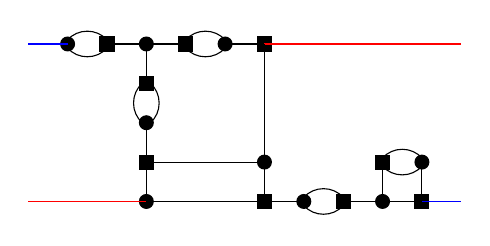
\begin{tikzpicture}[scale=0.5]
  \filldraw (0,0) circle (5pt);
  %\filldraw (0,1) circle (5pt);
  \draw[black, very thick, fill=black] (-0.15,0.85) rectangle (0.15,1.15);
  \filldraw (0,2) circle (5pt);
  %\filldraw (0,3) circle (5pt);
  \draw[black, very thick, fill=black] (-0.15,2.85) rectangle (0.15,3.15);
  \filldraw (0,4) circle (5pt);
  %\filldraw (0,5) circle (5pt);
  %\draw[black, very thick, fill=black] (-0.15,4.85) rectangle (0.15,5.15);
  \draw[black, very thick, fill=black] (-1.15,3.85) rectangle (-0.85,4.15);
  %\filldraw (-1,5) circle (5pt);
  \filldraw (-2,4) circle (5pt);
  %\filldraw (3,0) circle (5pt);
  \draw[black, very thick, fill=black] (2.85,-0.15) rectangle (3.15,0.15);
  %\filldraw (1,4) circle (5pt);
  \draw[black, very thick, fill=black] (0.85,3.85) rectangle (1.15,4.15);
  \filldraw (2,4) circle (5pt);
  %\filldraw (3,4) circle (5pt);
  \draw[black, very thick, fill=black] (2.85,3.85) rectangle (3.15,4.15);
  \filldraw (3,1) circle (5pt);
  \filldraw (4,0) circle (5pt);
  %\filldraw (5,0) circle (5pt);
  \draw[black, very thick, fill=black] (4.85,-0.15) rectangle (5.15,0.15);
  \filldraw (6,0) circle (5pt);
  %\filldraw (7,0) circle (5pt);
  \draw[black, very thick, fill=black] (6.85,-0.15) rectangle (7.15,0.15);
  %\filldraw (6,1) circle (5pt);
  \draw[black, very thick, fill=black] (5.85, 0.85) rectangle (6.15,1.15);
  \filldraw (7,1) circle (5pt);
  \draw[red] (-3,0) -- (0,0);
  \draw[red] (3,4) -- (8,4);
  %\draw[blue] (-2,5) -- (-1,5);
  \draw[blue] (-2,4) -- (-3,4);
  \draw[blue] (7,0) -- (8,0);
  \draw (0,0) -- (4,0);
  \draw (0,0) -- (0,2);
  \draw (0,3) -- (0,4);
  \draw (-1,4) -- (1,4);
  \draw (2,4) -- (3,4);
  \draw (0,1) -- (3,1);
  \draw (3,0) -- (3,4);
  \draw (5,0) -- (7,0);
  \draw (6,0) -- (6,1);
  \draw (7,0) -- (7,1);
  %\draw (-0.1,2) -- (-0.1,3);
  \draw (-0.1,2) .. controls (-0.4,2.25) and (-0.4,2.75) .. (-0.1,3);
  %\draw (0.1,2) -- (0.1,3);
  \draw (0.1,2) .. controls (0.4,2.25) and (0.4,2.75) .. (0.1,3);
  %\draw (-1, 4.9) -- (0,4.9);
  %\draw (-1,5.1) -- (0,5.1);
  %\draw (1,3.9) -- (2,3.9);
  \draw (1,3.9) .. controls (1.25,3.6) and (1.75,3.6) .. (2,3.9);
  %\draw (1,4.1) -- (2,4.1);
  \draw (1,4.1) .. controls (1.25,4.4) and (1.75,4.4) .. (2,4.1);
  %\draw (4,-0.1) -- (5,-0.1);
  \draw (4,-0.1) .. controls (4.25,-0.4) and (4.75,-0.4) .. (5,-0.1);
  %\draw (4,0.1) -- (5,0.1);
  \draw (4,0.1) .. controls (4.25,0.4) and (4.75,0.4) .. (5,0.1);
  %\draw (6,0.9) -- (7,0.9);
  \draw (6,0.9) .. controls (6.25,0.6) and (6.75,0.6) .. (7,0.9);
  %\draw (6,1.1) -- (7,1.1);
  \draw (6,1.1) .. controls (6.25,1.4) and (6.75,1.4) .. (7,1.1);
  \draw (-1,4.1) .. controls (-1.25,4.4) and (-1.75,4.4) .. (-2,4.1);
  \draw (-1,3.9) .. controls (-1.25,3.6) and (-1.75,3.6) .. (-2,3.9);
  \end{tikzpicture}
  \captionsetup{justification=centering}
  \caption{The cross-over-pinned-0 gadget $\mathcal{P}$}
  \label{a nice gadget}
\end{figure}
\begin{theorem}\label{thm:[0,1,0,0]}
The problem $\plholant{[0,1,0,0]}{(=_3)}$ is \numP-complete.
\end{theorem}



\begin{proof}
In~\cite{DyerF86}, Dyer and Frieze 
proved the problem Planar-X3C  NP-complete: An input is a
collection $\cal S$ of 3-element subsets of a set $U$, where the 
bipartite incidence graph is planar, and we ask for
an exact cover of $U$ by some ${\cal S'} \subseteq {\cal S}$.
Their reduction in fact produces instances 
where every $x \in U$ appears in exactly two or three sets of $\cal S$.
One can further verify that their reduction is parsimonious.
Thus, their proof yields the \#P-completeness for
$\plholant{[0,1,0,0],[0,1,0]}{(=_3)}$.
We prove our theorem by a reduction
\begin{equation}\label{reduction-in-thm4}
\plholant{[0,1,0,0],[0,1,0]}{(=_3)}\leq_{T} \plholant{[0,1,0,0]}{(=_3)}.
\end{equation}


Note that a unary pin-0 signature $\Delta_0$
connected to
$[0,1,0,0]$  produces $[0,1,0]$. If we replace  each $[0,1,0]$ in  $\Omega$ by 
 $[0,1,0,0]$ connected with  $\Delta_0$, the Holant value is unchanged.  
 So  if 
we can produce 
 $\Delta_0$ on the RHS in  $\plholant{[0,1,0,0]}{(=_3)}$, then (\ref{reduction-in-thm4}) follows. 
 But, in any bipartite 3-regular
problem 
\emph{provably} no construction can produce
individual unary signatures.  
Next, 
 note that in any signature grid $\Omega$ of  $\plholant{[0,1,0,0],[0,1,0]}{(=_3)}$,
 the number of  appearances of $[0,1,0]$ is congruent to $0 \bmod 3$, by counting the total degrees of LHS and RHS. Then, our idea is to create  triples of $\Delta_0$ so that we can apply them, one triple 
 at a time.
 

There remains the difficulty of how to construct  triples of $\Delta_0$ on the RHS in the  setting
 $\plholant{[0,1,0,0]}{(=_3)}$, and more importantly, not only the construction must be
 planar but also we must be able to apply them in $\Omega$, three at a time,
 in a planar fashion.  Notice that the appearances of $[0,1,0]$ in  $\Omega$ 
 generally do not allow this planar grouping (and indeed the output instances
 in~\cite{DyerF86} do not have this property).
 
The following construction accomplishes all these requirements in one fell swoop!
The planar cross-over-pinned-0 gadget $\mathcal{P}$ is illustrated in Figure~\ref{a nice gadget}, where we place  $[0,1,0,0]$ at the squares and  $=_3$ at the circles. It has the following properties:
\begin{enumerate}
    \item externally the two left dangling edges are to be connected to LHS, and two right dangling edges are to be connected to RHS;
    \item the two blue dangling edges are pinned to be 0;
    \item the two red dangling edges can be assigned to either 0 or 1, but must be the same value, and either choice
    induces  a unique assignment for the internal edges.
   % \item the gadget is planar.
\end{enumerate}
Note also that if we ``flip'' $\mathcal{P}$ along the ``axis'' of the two blue edges,
thereby exchange the two red edges, we have a reflected copy of $\mathcal{P}$,
call it  $\mathcal{P}'$,
where the North-East red edge connects externally to LHS, and the
South-West red edge connects externally to RHS, exactly the opposite of  $\mathcal{P}$.

Thus, the gadget  $\mathcal{P}$   allows ``passing over'' one crossing edge (the pair of
red edges will  take its place) 
while the two end blue edges are pinned to 0. 
We can link any $k \ge 1$ copies of   $\mathcal{P}$ or  $\mathcal{P}'$
by the blue edges to ``pass over''  $k$ crossings. Note that the linking of the 
two end blue edges respects the bipartite structure, and  $\mathcal{P}$ or  $\mathcal{P}'$
allow any individual bipartite orientation of the crossed edge.
We call this a linked  $\mathcal{P}$ gadget.

Let $n=3m$ be the number of $[0,1,0]$ in $\Omega$ for some integer $m\ge 0$.  We now add $m$ new vertices on RHS assigned the signature $=_3$. We then use three copies of the linked
 $\mathcal{P}$ gadgets to connect  this $=_3$ to three occurrences of $[0,1,0]$ in $\Omega$, while 
replacing  the signatures there by $[0,1,0,0]$.
(If  some passage from $=_3$ to  $[0,1,0]$ does not encounter any crossing edge, we will
artificially introduce two such crossings!)
This defines a signature grid $\Omega'$ in $\plholant{[0,1,0,0]}{(=_3)}$
with  $\operatorname{Holant}(\Omega') = \operatorname{Holant}(\Omega)$.
\end{proof}

\begin{remark}
One can easily construct a degenerate ternary signature $[1,0,0,0] = [1,0] \otimes [1,0] \otimes [1,0]$ on RHS by placing circles to be $[0,1,0,0]$ and squares to be $(=_3)$ on $G_2$. However, we cannot  apply Theorem~\ref{thm:P3EM} and conclude that 
$\plholant{[0,1,0,0],[0,1,0]}{(=_3)} \leq_{T} 
\plholant{[0,1,0,0]}{(=_3)}.$
% JYC pl check
%\plholant{[0,1,0,0]}{(=_3),[1,0,0,0]},$$
See also Remark~\ref{remark8}.
%after Lemma 4.4.
%in full paper attached. 
\textbf{The use of the gadget $\mathcal{P}$ is essential.}
%this yields an even simpler proof. However, we don't have such a reduction. In fact, if one turns to the gadget given by Dyer and Frieze in their parsimonious reduction to $\plholant{[0,1,0,0]}{(=_3),[1,0]}$, there is no planar way to assign an additional edge for each node with degree 2 into one of its adjacent faces so that every face has $0 \pmod{3}$ edges coming in if there exists a variable in the original Planar 1-SAT problem which appears only complemented or only uncomplemented as defined in~\cite{DyerF86}. 
\end{remark}



% \begin{proof}
% Consider the signature $[3b^2, 1+2b^3, 2b+b^4, 3b^2]$ on LHS which is obtained by placing squares to be $[0,1,b,0]$ and circles to be $=_3$ in $G_2$. Lemma~\ref{lemma:basic} applies (after normalizing) and the problem is \numP-hard unless $[3b^2, 1+2b^3, 2b+b^4, 3b^2]$  is degenerate or it satisfies $1+2b^3=2b+b^4$. Both cases will lead to $b=1$, in which case the problem $\plholant{[0,1,1,0]}{(=_3)}$ is the Pl-{\sc \#HyperGragh-Moderate-3-Cover} problem in~\cite{FanC21} and it was shown to be in $\operatorname{FP}$.
% \end{proof}

\section{Main Theorem}
We are now ready to prove our main theorem. At the end
of the proof there is a flowchart of the logical structure for this proof of
Theorem~\ref{thm:main}.

 \begin{proof}[Proof of Theorem~\ref{thm:main}]
 First, if $f_0 = f_3 = 0$, we separate the discussion into whether $f_1 f_2 \neq 0$. If $f_1 f_2 \neq 0$, by Theorem \ref{0ab0}  we know that it is  \numP-hard unless $f_1=f_2$, in which case it is matchgate-transformable and thus in FP. If $f_1 f_2 =0$, then by Theorem~\ref{thm:[0,1,0,0]} we know that it is  \numP-hard unless $f_1=f_2=0$, in which case the problem is trivially in FP. This finishes the case when $f_0 = f_3 = 0$.
  
 Assume now at least one of $f_0$ and $f_3$ is not $0$. 
% MK 16
 By considering the reversal of the signature, % flipping the role of 0 and 1,
 we can assume $f_0\ne 0$, then the signature becomes $[1,a,b,c]$ after normalization. 
 
 If $c=0$, the dichotomy for $[1,a,b,0]$ is proved in Theorem \ref{1ab0}.
 
 If in $[1,a,b,c]$, $c\ne 0$, then $a$ and $b$ are symmetric by flipping. Now if $ab=0$, we can assume $b=0$ by the afore-mentioned symmetry, i.e., the signature becomes $[1,a,0,c]$. By Theorem \ref{1a0c}, it is \numP-hard unless $a=0$, in which case it is Gen-Eq. 
 
 Finally, for the problem $[1,a,b,c]$ where $abc\ne0$, Theorem \ref{large5} proves the dichotomy that it is \numP-hard unless the signature is in the tractable cases of Theorem~\ref{thm:main}.
 \end{proof}


\bigskip  
\newpage
\textbf{Flowchart of proof structure: }

\medskip

\tikzstyle{startstop} = [rectangle, rounded corners, minimum width=2cm, minimum height=1cm,text centered, draw=black, fill=red!20]
\tikzstyle{io} = [trapezium, trapezium left angle=70, trapezium right angle=110, minimum width=3cm, minimum height=1cm, text centered, draw=black, fill=blue!20]
\tikzstyle{process} = [rectangle, minimum width = 2cm, minimum height=1cm, text centered,text width=2cm, draw=black, fill=yellow!20]
\tikzstyle{decision} = [diamond, minimum width=3cm, minimum height=1cm, text centered, draw=black, fill=green!20]
\tikzstyle{arrow} = [thick,->,>=stealth,  text centered, text width=2.2cm]

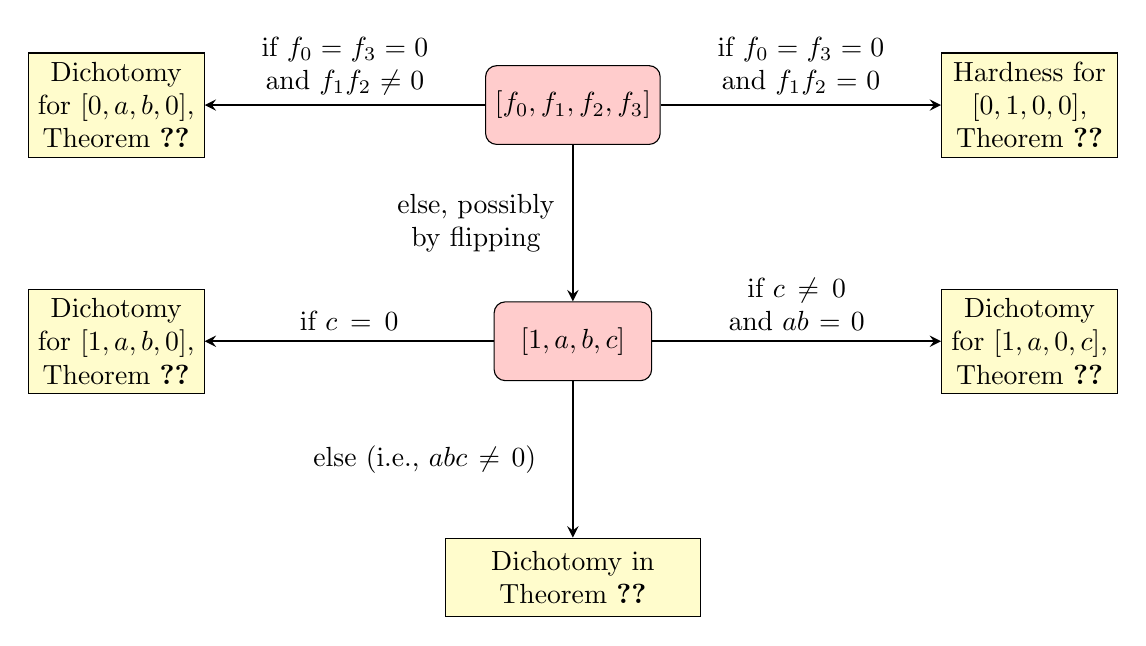
\begin{tikzpicture}[node distance=4cm]
    \node (s1) [startstop] {$[f_0,f_1,f_2,f_3]$};
    \node (s2) [process, left of=s1, xshift=-1.8cm] {Dichotomy for $[0,a,b,0]$, Theorem~\ref{0ab0}};
    \node (s3) [startstop, below of=s1, yshift=1.0cm] {$[1,a,b,c]$};
    \node (s4) [process, left of=s3,xshift=-1.8cm] {Dichotomy for $[1,a,b,0]$, Theorem~\ref{1ab0}};
    \node (s5) [process, right of=s3, xshift=1.8cm] {Dichotomy for $[1,a,0,c]$, Theorem~\ref{1a0c}};
    \node (s6) [process, below of=s3, yshift=1.0cm, text width=3cm] {Dichotomy in Theorem~\ref{large5}};
    \node (s7) [process, right of=s1, xshift = 1.8cm] {Hardness for $[0,1,0,0]$, Theorem~\ref{thm:[0,1,0,0]}};
    
    \draw [arrow] (s1) -- node[anchor=south] {if $f_0=f_3=0$ and $f_1 f_2 \neq 0$} (s2);
    % \draw [arrow] [text width=3.8cm](s1) -- node[anchor=west] {else, possibly by flipping} (s3);
    \draw [arrow] (s1) -- node[anchor=east] {else, possibly by flipping} (s3);
    \draw [arrow] (s3) -- node[anchor=south] {if $c=0$} (s4);
    \draw [arrow] (s3) -- node[anchor=south] {if $c \ne 0$ and $ab=0$ } (s5);
    \draw [arrow] [text width =3.5cm](s3) -- node[anchor=east] {else (i.e., $abc\ne 0$)} (s6);
    \draw [arrow] (s1) -- node[anchor=south] {if $f_0=f_3=0$ and $f_1 f_2 = 0$} (s7);
\end{tikzpicture}

% \section*{References}

